% !TeX spellcheck = en_US
\documentclass[AIRstudentthesis%      style
,optCharter%            font
,optBlackHeadings%      black sections to reduce number of colored pages
,optBlackRefs%          black references to reduce number of colored pages
%,optCMYK%              color model
,optBiber%              bibliography tool
,optBibstyleAlphabetic% bibliography style
,optCenterEquations%    alignment of equations
,optEnglish%            language
%,optTikzExternalize%   compiles faster for large tikz images
,optComputerModernMath
]{AIRlatex}


% Load additional LaTeX packages - remove what you do not need
\usepackage{algorithm}
\usepackage{algorithmicx}
\usepackage{booktabs}
\usepackage{upgreek}
\usepackage{todonotes}
\usepackage{textcomp}
\usepackage{comment}
\usepackage{subcaption}
\usetikzlibrary{angles, quotes}

% Set paths
\graphicspath{{figures/}}
\addbibresource{source/literature.bib}

% Define additional commands
\newcommand{\code}[1]{\texttt{#1}}
\newcommand{\degree}[0]{^\circ}

\begin{document}
    % Titlepage
    \frontmatter
    \AIRstudentthesisTitlePageCustomBachelorsThesis{Aktive taktile Erkundung auf der Grundlage eines schnurrhaar-inspirierten Sensorarrays}{Active Tactile Exploration Based on \\ Whisker-Inspired Sensory Array}{\AIRlangFieldOfStudyRoboticsCognitionIntelligence}{Valentin Safronov}{}{\AIRnamesProfKnoll}{Yixuan Dang, M.Sc.}{\AIRutilsDate{28}{03}{2025}}

    % Abstract
    % In total max. 1 Page!
\AIRstudentthesisAbstract{
    Object contour reconstruction is critical in robotics for tasks such as navigation and recognition.
    Whisker sensors offer a promising tactile modality due to their high spatial resolution, robustness under varying conditions, and low computational requirements.
    However, existing approaches typically fail to reconstruct objects with sharp corners, as the whisker detaches from the object, and do not allow for contour reconstruction in confined spaces.
    In this work, we introduce a development platform that integrates multiple magnetically transduced whisker sensors, mounted on a robotic arm for active control.
    For single-whisker configurations, we propose an enhanced contour-following strategy paired with an object retrieval policy to manage unavoidable whisker detachments at sharp corners and accurately capture their contours.
    For multi-whisker setups, a tunneling policy is introduced, and all control policies are combined into a single finite state machine that dynamically selects the active policy and determines which whiskers are relied on.
    Simulation results demonstrate that our method effectively reconstructs contours with sharp angles, and maintains a centered trajectory in confined passages.
    Finally, we present a comprehensive framework for real-world experiments, including data collection, preprocessing, evaluation, storage, and visualization.
}{
    Die Rekonstruktion von Objektkonturen ist in der Robotik für Aufgaben wie Navigation und Erkennung von entscheidender Bedeutung.
    Schnurrbart-Sensoren bieten aufgrund ihrer hohen räumlichen Auflösung, Robustheit unter wechselnden Bedingungen und geringem Rechenaufwand eine vielversprechende taktile Modalität.
    Bestehende Ansätze scheitern jedoch typischerweise daran, Objekte mit scharfen Ecken zu rekonstruieren, da sich der Schnurrbart vom Objekt löst, und erlauben keine Konturrekonstruktion in engen Räumen.
    In dieser Arbeit stellen wir eine Entwicklungsplattform vor, die mehrere magnetisch transduzierte Schnurrbart-Sensoren integriert, die auf einem Roboterarm für aktive Steuerung montiert sind.
    Für Einzel-Schnurrbart-Konfigurationen schlagen wir eine verbesserte Konturverfolgungsstrategie in Kombination mit einer Objekt-Rückholpolitik vor, um unvermeidliche Schnurrbartablösungen an scharfen Ecken zu handhaben und deren Konturen präzise zu erfassen.
    Für Mehr-Schnurrbart-Systeme wird eine Tunneling-Politik eingeführt, und alle Steuerungsstrategien werden in einer einzigen endlichen Zustandsmaschine kombiniert, die dynamisch die aktive Strategie auswählt und bestimmt, auf welche Schnurrbärte vertraut wird.
    Simulationsergebnisse zeigen, dass unsere Methode Konturen mit scharfen Winkeln effektiv rekonstruiert und eine zentrierte Bahn in engen Passagen beibehält.
    Abschließend präsentieren wir ein umfassendes Framework für reale Experimente, einschließlich Datenerfassung, Vorverarbeitung, Evaluierung, Speicherung und Visualisierung.
}


    % Content
    \AIRstudentthesisPrintTableOfContents
    \mainmatter
    % !TeX spellcheck = en_US


\chapter{Introduction}


\section{Biological Whiskers}

Over the past two decades, tactile perception has gained attention within robotics, a field traditionally dominated by visual sensing~\cite{s22072705}.
Tactile sensing provides distinct advantages, especially when visibility is limited, in low-light conditions, or when environments are narrow, cluttered, or visually obstructed.
Nature provides ample evidence of the effectiveness of tactile sensing and offers inspiration for the development of tactile sensors.

Some animals possess tactile sensory hairs known as whiskers or vibrissae, which complement their vision.
Whiskers enable them to interact effectively with their environment through non-intrusive mechanical contact.
\enquote{Traditionally, whiskers are associated with diverse survival skills, including tactile discrimination, distance assessment, food acquisition, gap crossing, and social interaction} note Ibarra-Castaneda et al.~\cite{IBARRACASTANEDA2022100034}.
For example, seals and sea lions use their whiskers for hunting in dark and turbid environments.
When prey swims nearby, the generated hydrodynamic vortices cause distinct, jerky deflections in the whiskers.
These deflections reveal the hydrodynamic trail left by the prey, allowing seals and sea lions to locate their prey effectively~\cite{muthuramalingam2018sealsealionwhiskers}.
Thus, whiskers function as passive sensors by responding directly to external excitation.

In contrast, some rodents such as rats and squirrels can move their whiskers actively, in rhythmic motions known as \textit{whisking}, enabling them to actively perceive their immediate surroundings and to distinguish surface textures.
Different textures produce unique slip-stick motion patterns and deflection magnitudes of whiskers, resulting in characteristic resonant vibrations that rodents interpret to identify surfaces and objects~\cite{wolfe2008texture}.

Rats particularly depend on whisker-based navigation when traversing confined spaces, such as tunnels or burrows.
Through coordinated whisking motions, rats efficiently detect the layout and contours of the environment, allowing them to move even in complete darkness~\cite{*}.

The anatomical structure and functional mechanisms of biological whiskers are depicted in Figure~\ref{fig:whisker-anatomy}.
Whiskers come in various shapes and sizes, and one animal can have multiple whiskers, each with a different length and taper.
Sensory detection is carried out solely by mechanoreceptors located at the base of each whisker follicle, without any additional receptors along the whisker shaft~\cite{doi:10.1089/soro.2016.0028}.
This simplicity, effectiveness and variability of biological whiskers provides a foundation for developing biomimetic tactile sensors.

\begin{figure}[htb]
    \centering
    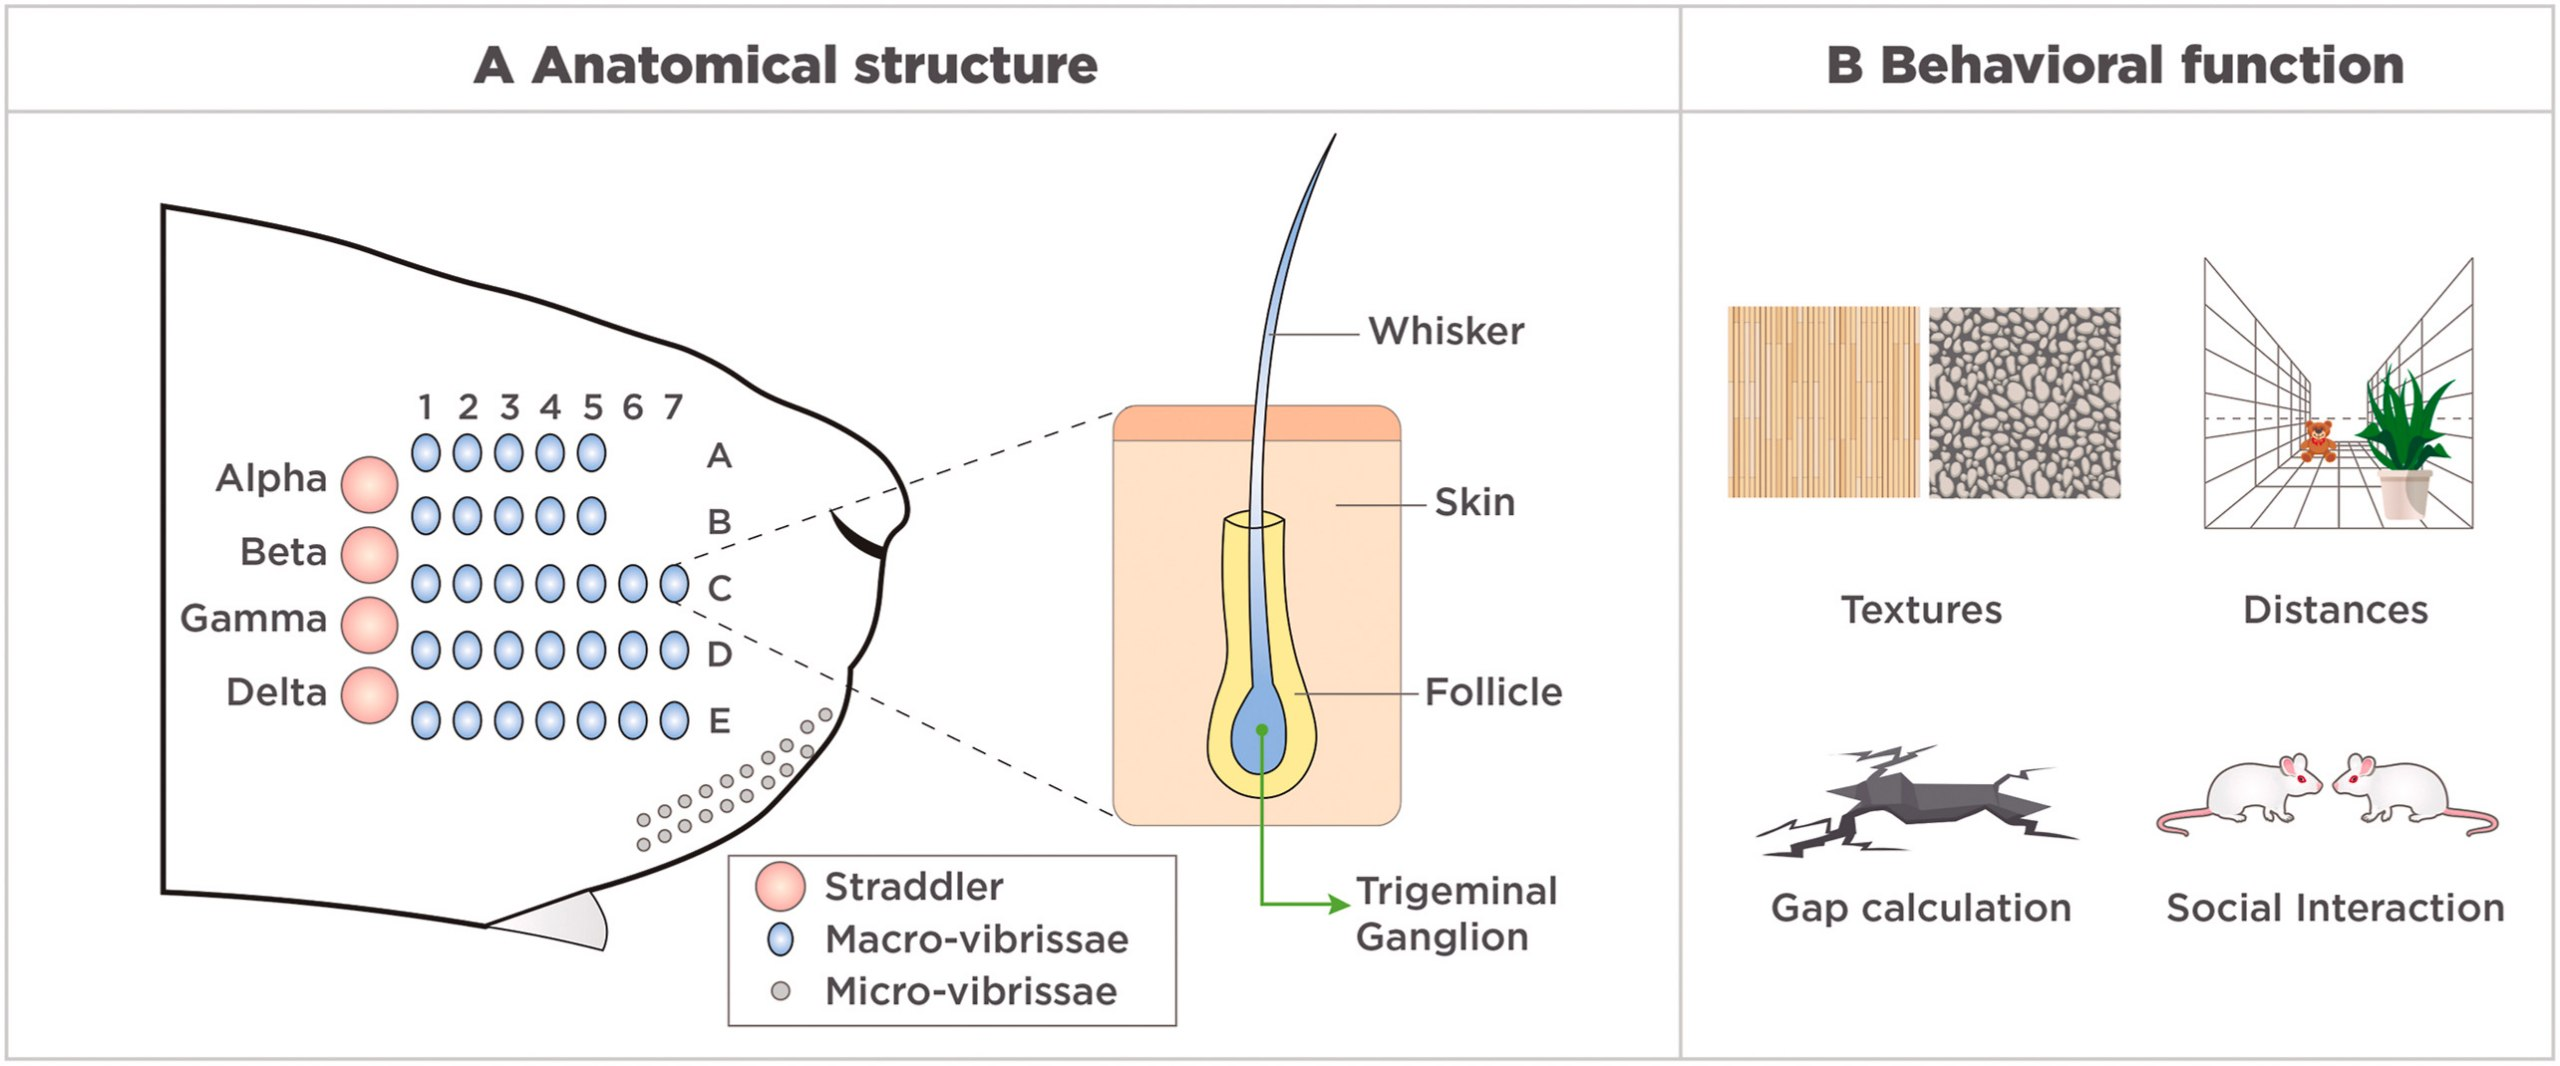
\includegraphics[width=\textwidth]{figures/whisker-anatomy}
    \caption{Representation of the vibrissae system and its function, from~\cite{IBARRACASTANEDA2022100034}}
    \label{fig:whisker-anatomy}
\end{figure}


\section{Whisker-inspired Tactile Sensors}

The versatility and effectiveness of biological whiskers have inspired numerous developments in the field.
Whisker-inspired tactile sensors have extensive applications, including~\cite{s22072705}:
\begin{itemize}
    \item Recognition of the surrounding objects and obstacle avoidance (extraction of the 3D whisker tip position)
    \item Exploration of unstructured environments
    \item Leak detection in pipelines
    \item Water flow detection in unmanned underwater vehicles
    \item Midair obstacle detection for drones
    \item Tactile sensing of heart valves
    \item Navigation in dark or visually obscured environments
    \item Study of the surface texture (like surface hardness and adhesiveness of food)~\cite{https://doi.org/10.1002/aisy.202300660}
\end{itemize}

Whisker-inspired tactile sensors offer low power consumption, minimal computational requirements, and high spatial resolution.
Some of the most commonly used whisker-inspired tactile sensors are:~\cite{s22072705}
\begin{itemize}
    \item \textbf{Strain gauge sensors:} measure changes in electrical resistance caused by deformation of strain gauges attached to the whisker shaft.
    \item \textbf{Hall effect sensors:} detect changes in magnetic field strength caused by displacement or rotation of the magnet positioned at the whisker base.
    \item \textbf{Capacitive sensors:} detect changes in capacitance caused by deformation of the whisker.
    \item \textbf{Piezoelectric sensors:} generate an electrical charge in response to mechanical stress applied to the whisker.
    \item \textbf{Optical sensors:} change light path or intensity as the fiber-based whisker deflects.
    \item \textbf{Magnetoresistive sensors:} measure changes in electrical resistance caused by changes in magnetic fields when whisker deflection occurs.
    \item \textbf{MEMS-based sensors:} employs a capacitive or piezoelectric sensor in a microelectromechanical system format.
\end{itemize}
Taxonomy of whisker sensors is shown in Figure~\ref{fig:taxonomy}.

\begin{figure}[htb]
    \centering
    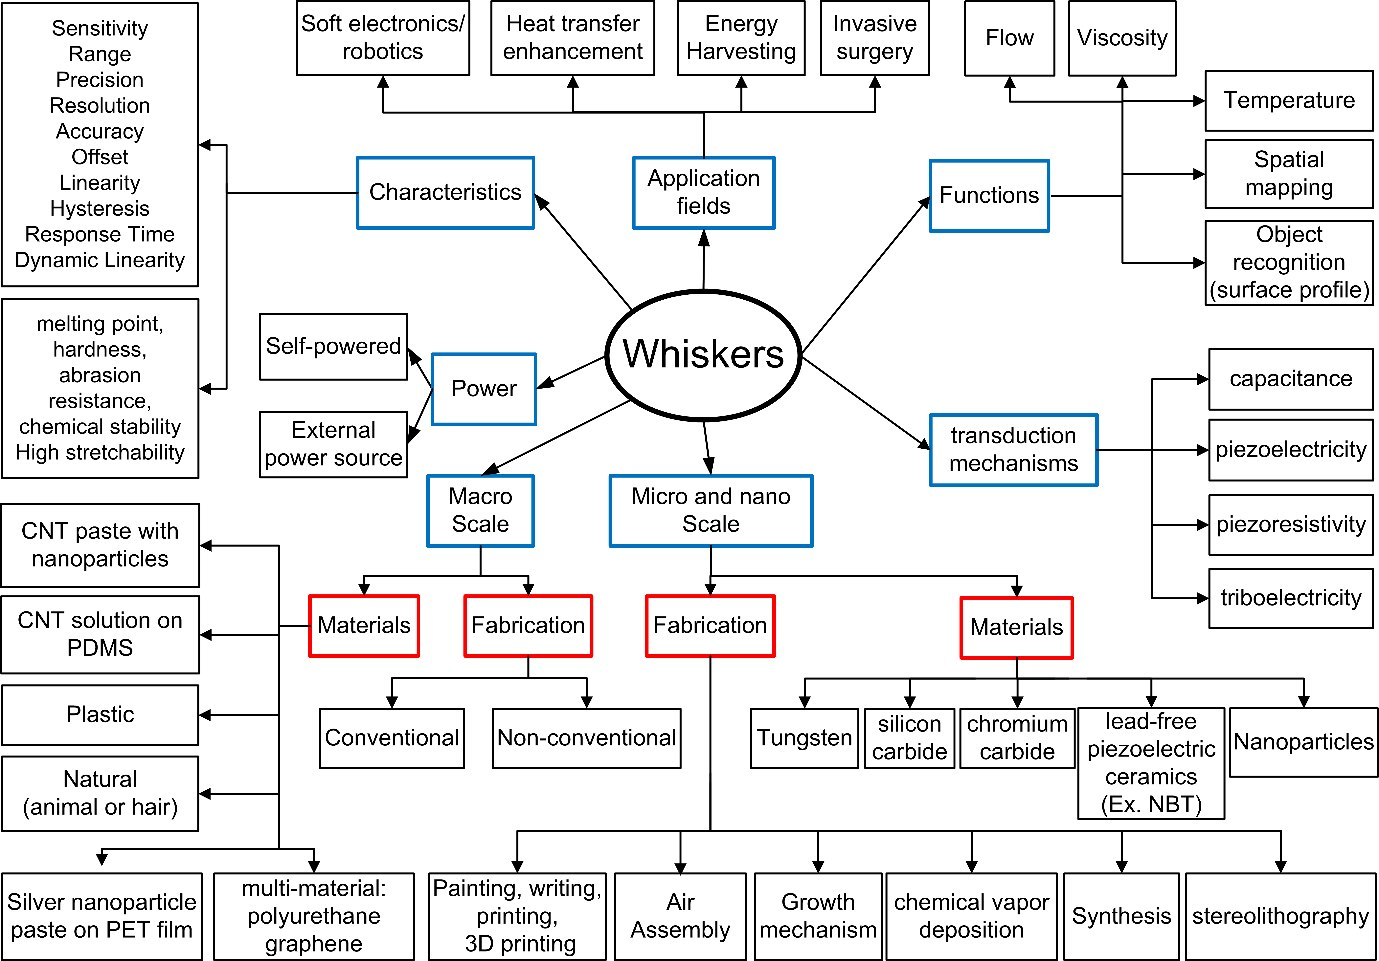
\includegraphics[width=0.65\textheight]{figures/taxonomy}
    \caption{A taxonomy for whisker-based sensors, from \cite{s22072705}}
    \label{fig:taxonomy}
\end{figure}


\section{Active Tactile Perception}
One of the most critical problems in robotics is \textbf{reconstruction of unstructured environments}.
It is essential for efforts to develop \textbf{autonomous mobile manipulators}, that are said to have significant societal and economic impact~\cite{how-can-robots-succeed}.
Operation in unstructured environments poses multiple challenges, such as:~\cite{how-can-robots-succeed}
\begin{itemize}
    \item Limited knowledge of the surroundings
    \item Uncertainty in the robot's position
    \item Constraints on the robot's mobility
    \item Impermanence of the state of the environment
\end{itemize}
Thus, the reconstruction of unstructured environments plays a pivotal role in the robot's ability to navigate and manipulate objects in its environment.

Whisker sensors are particularly well-suited for this task due to their \textbf{non-intrusive nature} and \textbf{reconstruction precision}.
They can be attached to the autonomous mobile manipulator, providing it with tactile information for accurate environment reconstruction, navigation and obstacle avoidance.
Furthermore, they are lightweight and low-cost, making them suitable for integration into small robots.

However, the use of whisker sensors for active tactile perception poses several challenges.
For single whisker configurations the following challenges arise:
\begin{itemize}
    \item The whisker requires \textbf{active control} to maintain contact with the object.
    \item \textbf{The whisker might slip or detach} if the surface is uneven or rough, or when sharp corners are encountered.
    \item The whisker \textbf{must maintain a certain deflection profile} to ensure accurate measurements.
    \item The whisker mustn't be compressed or bent too much, as this can lead to damage or wear.
    \item The whisker can bend in the wrong direction, preventing further exploration until it is repositioned.
\end{itemize}

For platforms integrating multiple whiskers additional challenges arise:
\begin{itemize}
    \item The platform must be aware of its size and shape, as to not collide with the environment.
    \item The platform must be able to \textbf{navigate in confined spaces}, such as tunnels or narrow passages.
    \item The platform must follow the above-mentioned requirements for each whisker.
\end{itemize}

To circumvent these challenges, a robust platform and control system is required.


\section{Overview of the Thesis}

\textbf{This thesis focuses on the use of whisker sensors for active tactile perception in unstructured environments.
We aim to develop a control algorithm that allows a robotic platform to actively explore and reconstruct its environment using whisker sensors.}
First, a \textbf{simulation framework based on MuJoCo} is developed to test the proposed control algorithms.
The whisker shaft is simulated as a composite of 40 elastic cables.
The whisker contacts with the objects are assumed to be frictionless.
A massive platform with two integrated whisker from left and right sides is set up for active control.

The control system is build upon specialized control policies for different tasks.
It accepts platform position and rotation as inputs and outputs platform linear and angular velocity.
It runs at a \textbf{frequency of 30 Hz}.
Platform linear velocity is always pointing at the target position, determined by the algorithm, with no smoothing or filtering.
For angular velocity a \textbf{PID controller} driven by the platform yaw error is employed.

The basic building block is the \textbf{swiping policy}, which enables a single whisker to follow smooth contour of an object.
It balances between preserving optimal whisker deflection and following the object's surface tangentially.
Without the desired deflection the whisker will either detach or measure with low accuracy.
The tangential contour tracking is required to ensure a steady direction of movement, as the deflection compensation per se does not imply any movement or a certain direction.
The swiping policy is tested in simulation on various objects, including a disk, a rectangular box with rounded corners and an object with moderate inflections.
The swiping policy achieves \textbf{submillimeter accuracy} on all tests and is shown to pass angles of \textbf{up to 30\degree without detaching}.

After that we introduce the \textbf{retrieval policy}, which allows the whisker to reattach to the object if it detached at a sharp corner.
It aims to reconstruct the edge contour and to revert to the swiping policy.
In order to do so, it tries for a contact a certain distance away from the edge, at a certain angle, until it comes into contact with the object.
This contact at the opposite side of the edge is used to determine the edge angle.
As edge reconstruction is required, the whisker swipes back to the edge until it detaches, then the platform reorients and approaches the edge again, now properly aligned.
Once a steady contact is established, the control is switched back to the swiping policy.
The retrieval policy is tested in simulation on various objects, including an octagon, a cube, a prism and a wall.
It consistently succeeded in reattaching the whisker to the object and reconstructing the edge contour, delivering the average reconstruction error of 1mm.
The retrieval policy is shown to handle the entire range of corner angles, from 30\degree to 180\degree and to stick to the defined retrieval radius of 1cm.
It generates a stable platform trajectory, only slightly diverging from the ideal trajectory, which would assume no whisker detachment and immediate reorientation at the edge.

\section{Key Contributions}

\begin{enumerate}
    \item We present a new \textbf{whisker sensor array} design using magnetically transduced whiskers, with 3 whiskers on each side of the platform.
    \item We introduce \textbf{Swiping policy} for uninterrupted contour tracking, achieving a submillimeter accuracy.
    It balances between preserving optimal whisker deflection and following the object's surface tangentially.
    \item We propose \textbf{Retrieval policy} for object retrieval in case of whisker detachment at sharp corners, managing the entire range of corner angles and ensuring edge contour reconstruction.
    It involves edge angle resolution, whisking back and reattaching the whisker to the object.
    \item We develop a \textbf{Tunneling policy}, allowing navigation in tunnels, for multi-whisker setups and show that it is able to maintain a centered trajectory in confined passages.
    It aims to keep the whiskers in contact with the walls, while following the tunnel and avoiding collisions.
    \item Additionally, we prepare a \textbf{simulation framework} for the whisker control system to automate the testing of the control policies.
    MuJoCo physics engine is used to simulate the whisker sensor and the environment.
    \item Finally, we present a \textbf{system infrastructure} for real-time sensor data visualization and evaluation.
    It is designed to be modular and extensible, and provides functionality for active control, data collection, storage and visualization.
\end{enumerate}

    % !TeX spellcheck = en_US


\chapter{Related Works}


\section{Whisker-Inspired Tactile Sensors}
Several structural designs have been proposed for whisker sensors.
They mainly differ in their transduction principle: how the normal force of contact is transferred to the sensor base.
The most common designs use passive, flexible cantilever whiskers integrated with strain gauges or piezoresistive elements to measure deflections.
Capacitive and optical variants also exist but are less widely used.
Additionally, magnetically transduced whiskers, although less common in industry, offer a low-cost and easily manufacturable alternative~\cite{8968518}.

\subsection{Magnetically Transduced Whisker Sensors}
Although magnetically transduced whisker sensors have yet to be widely adopted, they provide high precision and sensitivity, making them suitable candidates for tactile sensing.
Kim et al.~\cite{8968518} developed a magnetically transduced whisker sensor using a small permanent magnet attached to a flexible, cantilevered whisker.
Figure~\ref{fig:kim-whisker} illustrates this sensor design.
Its operating principle is straightforward: when the whisker contacts an object, deflection shifts the magnet embedded in a compliant, spring-like suspension relative to a magnetic sensor.
The magnetic field strength is therefore proportional to the moment applied at the whisker base.
Calibration is performed by measuring sensor output at various deflection angles and fitting the data using Gaussian process regression.
One advantage is easy waterproofing, as the whisker does not directly contact the sensor.
A limitation, however, is the rigidity of the whisker, complicating surface tracking.

Dang et al.~\cite{dang2025whisker} introduced a magnetically transduced whisker sensor employing a flexible nitinol wire as the whisker.
They proposed a suspension device comprising three integrated, flexible spiral arms.
Their sensor structure, shown in Figure~\ref{fig:dang-whisker}, resembles Kim et al.'s design.
They assume tip contact and model the tip position based on the whisker's deflection profile, parameterized using the one-dimensional measurement from a Hall sensor along the respective axis.
A limitation of their approach is the indistinguishability of tip and tangential whisker contacts, as both produce identical deflection profiles at the whisker base.

\begin{figure}[htb]
    \centering
    \begin{subfigure}{0.48\textwidth}
        \centering
        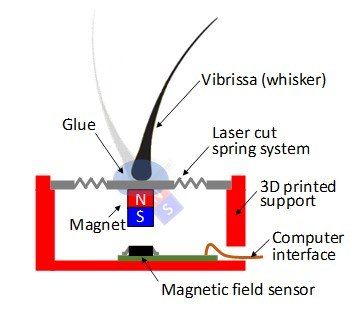
\includegraphics[width=\textwidth]{figures/kim-velez-whisker}
        \caption{Magnetically transduced whisker sensing mechanism schematic by Kim et al.~\cite{8968518}.}
        \label{fig:kim-whisker}
    \end{subfigure}\hfill
    \begin{subfigure}{0.48\textwidth}
        \centering
        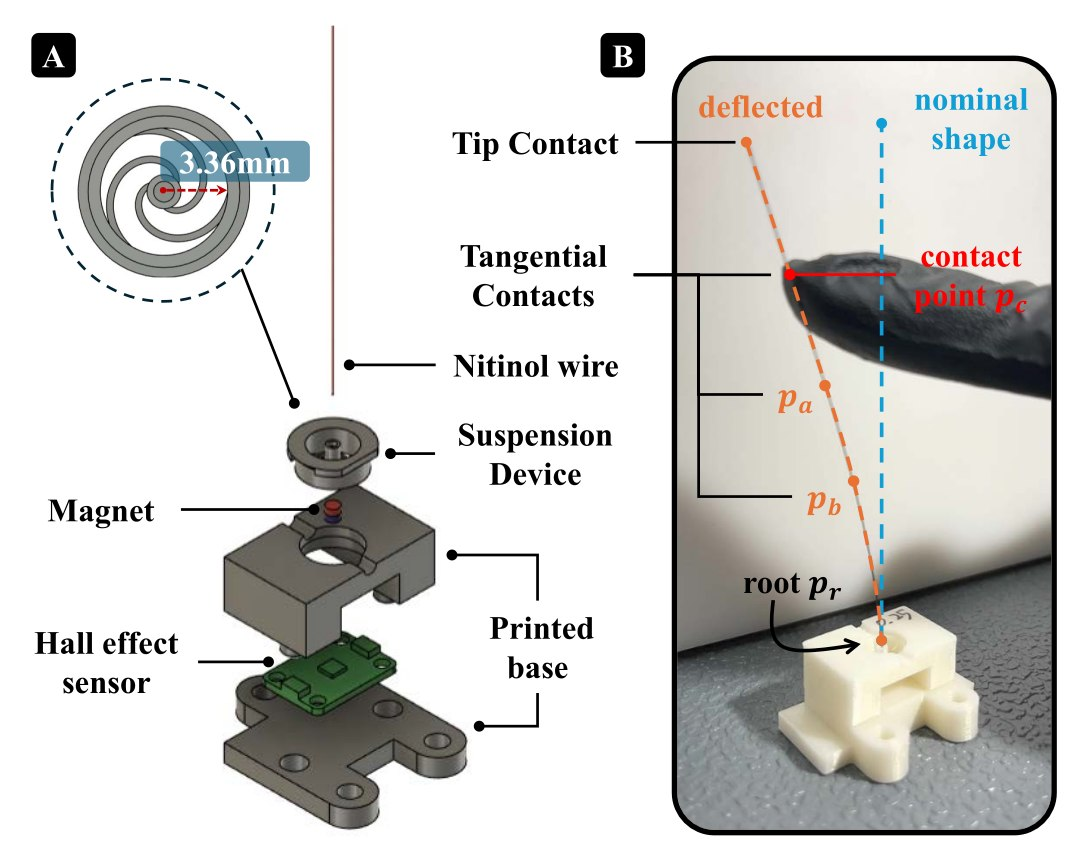
\includegraphics[width=\textwidth]{figures/dang-whisker}
        \caption{Structure of whisker-inspired tactile sensor by Dang et al.~\cite{dang2025whisker}.}
        \label{fig:dang-whisker}
    \end{subfigure}
    \caption{Side-by-side comparison of whisker sensor designs.}
\end{figure}

\subsection{Piezoresistive Whisker Sensors}
Piezoresistive whisker sensors are the most common type, notably applied in marine robotics to detect water flow and pressure variations.

Guo et al.~\cite{GUO2024114875} developed a piezoelectric wavy whisker sensor (PWWS) inspired by seal whiskers.
The sensor consists of a flexible, waterproof PDMS body and a thin sensing layer made of PVDF.
PDMS, a rubber-like material, protects the sensor from water, while PVDF is a polymer generating a small electrical voltage when bent or pressed.
When water flows around an object, vortices form, pushing against the whisker, bending the PVDF layer, and producing a voltage as depicted in Figure~\ref{fig:piezoelectric-whisker}.
The generated voltage correlates with water flow parameters, enabling tracking of underwater disturbances.

\begin{figure}[htb]
    \centering
    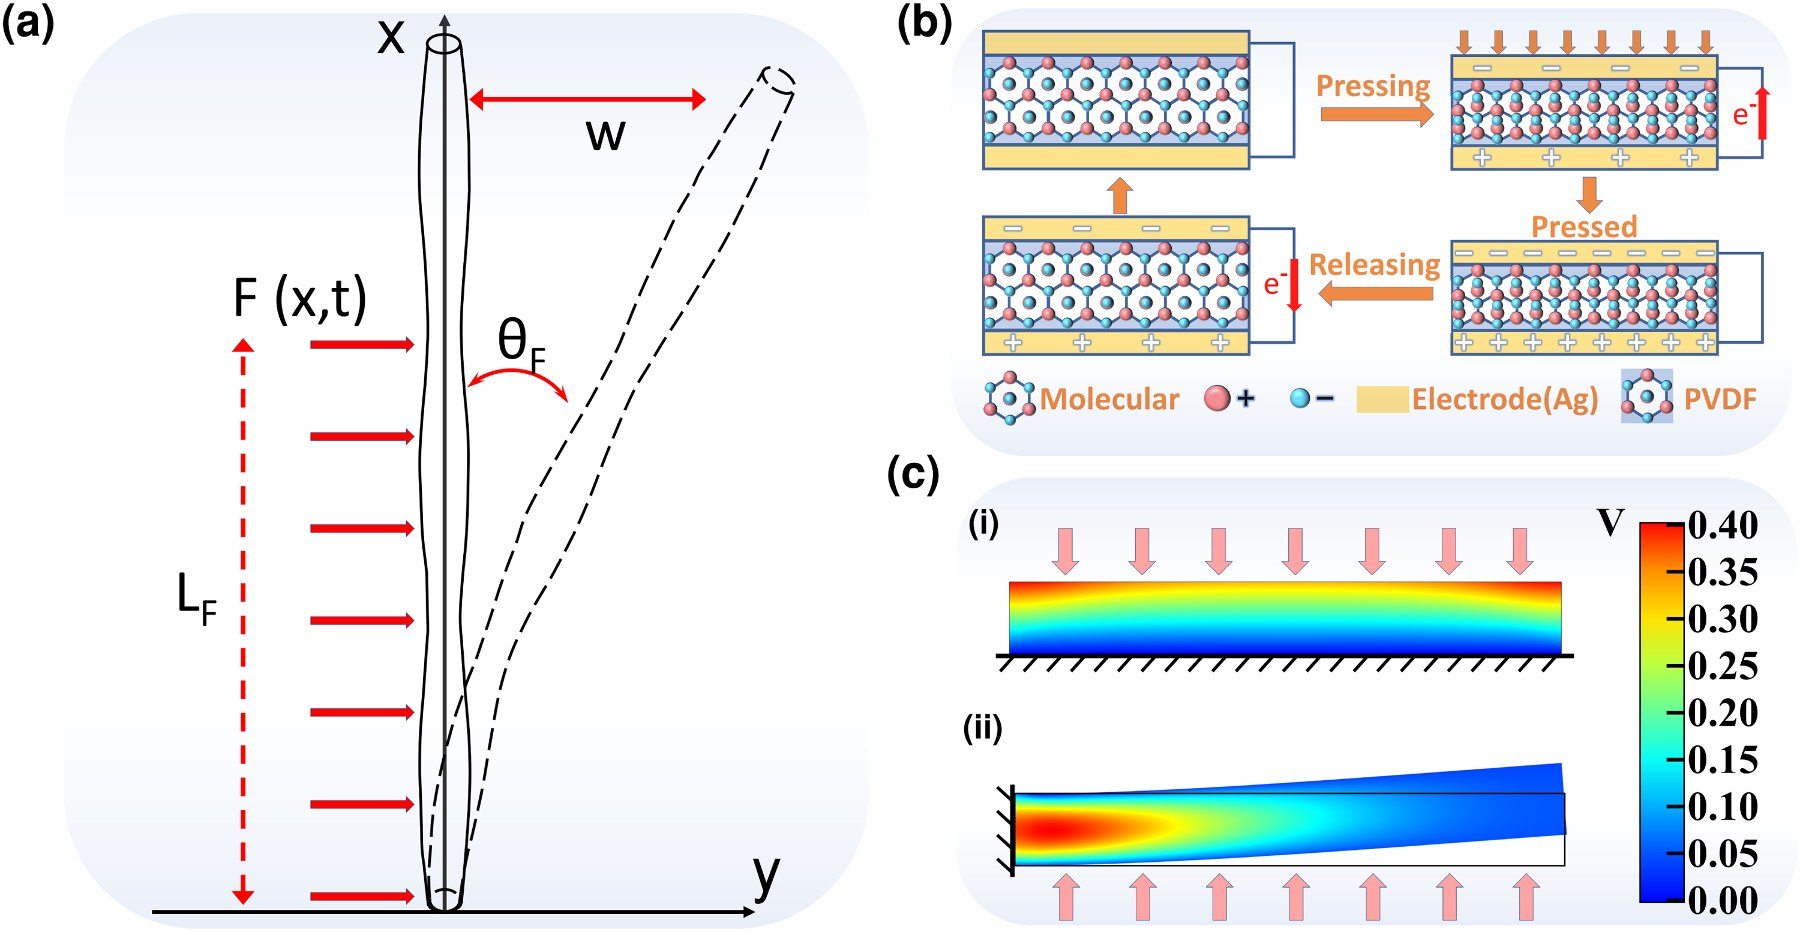
\includegraphics[width=\textwidth]{figures/piezoelectric-whisker}
    \caption{Operating principles of the PWWS by Guo et al.~\cite{GUO2024114875}. (a) Schematic of whisker deflection under force. (b) Cycle of electrical signals generated by the piezoelectric sensing unit. (c) Simulation of piezoelectric voltage within PVDF material under various constraints when subjected to external forces.}
    \label{fig:piezoelectric-whisker}
\end{figure}

\subsection{MEMS Whisker Sensors}
Wei et al.~\cite{9114501} developed a MEMS-based biomimetic whisker sensor replicating the tactile sensing mechanism of rats.
The sensor is integrated onto a small silicon chip (6.8\,mm square) containing four identical sensing units.
Each unit mimics the follicle arrangement of a rat's whisker, featuring a flexible whisker shaft attached to a central hub and four beams.
Piezoresistors implanted on these beams form a Wheatstone bridge.
Whisker bending from contact changes the resistance, producing an electrical signal.
The sensor fabrication uses standard MEMS processes, and the resulting structure is shown in Figure~\ref{fig:mems-whisker}.
Production begins with an SOI wafer, followed by ion implantation, insulating and metal layer deposition, and beam etching.
Experiments indicate the sensor reliably measures contact distances (30--40\,mm), recognizes object shapes (round, flat, beveled), and differentiates textures.
Thus, this whisker sensor has significant potential for integration into robotic systems requiring tactile sensing.

\begin{figure}[htb]
    \centering
    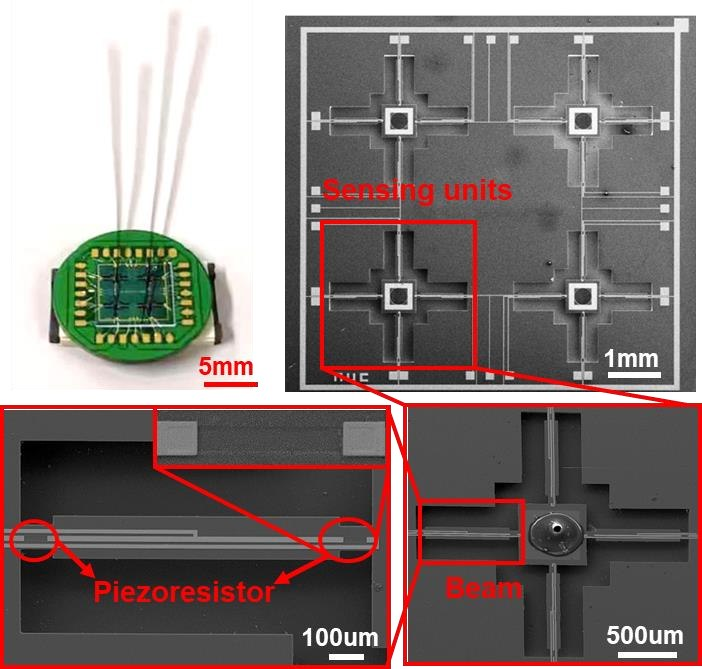
\includegraphics[height=0.4\textheight]{figures/mems-whisker}
    \caption{SEM image of the MEMS-based biomimetic whisker sensor by Wei et al.~\cite{9114501}.}
    \label{fig:mems-whisker}
\end{figure}


\section{Active Tactile Exploration}

This thesis is largely based on the work of Dang et al.~\cite{dang2025whisker}, who, besides the whisker sensor, also developed a control system for active tactile exploration.
They
\subsection{Previous Work}


    % !TeX spellcheck = en_US


\chapter{Hardware Design}

Hardware design goes here.
    % !TeX spellcheck = en_US


\chapter{Control Algorithms}

This chapter presents the control strategies that enable the whisker sensor system to accurately reconstruct object contours through tactile exploration.
It details a Finite State Machine (FSM) based framework that integrates multiple control policies: swiping for continuous contour tracking, retrieval for re-establishing lost contacts and tunneling for balanced navigation between surfaces.
The algorithms leverage real-time sensor feedback, spline-based trajectory planning, and PID-based body motion control to ensure smooth, adaptive interactions with diverse object geometries.


\section{Overview}

The whisker control algorithm is developed to reconstruct an object's contour by swiping along its surface.
Before we delve into the details of the control algorithm, we need to mention that its implementation is available on GitHub\footnote{\url{https://github.com/SVDouble/RatteChan}}.

The following key requirements were determined for the control model design:

\begin{enumerate}
    \item \textbf{Precise Contour Reconstruction:} The algorithm must accurately capture the local shape at the point of contact, ensuring that the detailed profile of the object is recorded.
    \item \textbf{Accurate Curve Following:} It must adeptly follow both smooth curves and sharp angles, all while maintaining an optimal whisker deflection.
    The constant whisker deflection is crucial for a predictable and small whisker tip position resolution by the deflection model.
    \item \textbf{Robust Detachment Recovery:} Sudden changes in the object's geometry can cause the whisker to detach.
    The system is, therefore, designed to quickly detect such events and recover contact with minimal disruption.
    \item \textbf{Collision Avoidance:} Considering the platform's dimensions, the algorithm incorporates measures to prevent collisions with the object during contour tracking.
\end{enumerate}

\noindent \textbf{Assumptions:} The development of this control strategy is based on the following assumptions:
\begin{enumerate}
    \item The contour is captured in a 2D (xy) plane, meaning that both the platform and whiskers operate with planar motion.
    \item All objects are rigid and remain stationary during the contact process.
    \item Contact occurs exclusively at the tip of the whisker.
    \item Forces exerted by the whiskers do not significantly affect the platform's motion.
    \item The platform's absolute position in the world frame is continuously known.
    \item The initial trajectory of the platform ensures that at least one whisker will eventually come into contact with the object.
    \item Although multiple objects may be present, the system focuses on a single object at any given time.
\end{enumerate}

\noindent To meet these requirements, the control algorithm is implemented as an FSM that sequences the following policies:

\begin{enumerate}
    \item \textbf{Swiping Policy:} The whisker performs a continuous swiping motion along the object's curve while maintaining an optimal deflection profile.
    \item \textbf{Retrieval Policy:} In the event of whisker detachment, this policy analyzes the detachment reason, re-establishes contact, and resumes the swiping motion, ensuring contour continuity.
    \item \textbf{Tunnelling Policy:} When operating between two surfaces, the algorithm maintains a centered trajectory, ensuring balanced contact on both sides.
\end{enumerate}

This structured approach enables the control system to dynamically adapt to varying contact scenarios.


\section{Variables}

It is necessary to consider the variables of the control algorithm.
Inputs come from three main sources:
\begin{enumerate}
    \item \textbf{Platform Sensors:} Provide the platform's position, orientation, and whisker deflection.
    \item \textbf{Geometric Configuration:} Information such as whisker placement.
    \item \textbf{Algorithm Configuration:} Parameters like the whisker deflection threshold.
\end{enumerate}
The output variables define the target linear and angular velocities of the platform.
A summary of these variables is provided in Table~\ref{tab:variables}.

\newcommand{\branch}[3]{%
    \scalebox{0.75}{$\left\{
                         \begin{array}{@{}l@{\quad}l@{}}
                             #2, & \text{if } #1,\\[0.5em]
                             #3, & \text{otherwise.}
                         \end{array}
    \right.$}%
}


\begin{table}[htb]
    \centering
    \begin{tabular}{p{1cm} p{2.2cm} p{3cm} p{7.8cm}}
        \toprule
        \textbf{Name}                                        & \textbf{Values}                                                   & \textbf{Source}                                         & \textbf{Description}                                                                                                        \\
        \midrule
        \multicolumn{4}{l}{\textbf{Control Inputs: Platform}} \\
        \midrule
        \(^{\mathrm{w}}\boldsymbol{r}^{t}\)                  & \(\mathbb{R}^2, [x, y]^\mathrm{T}\)                               & Measured                                                & Radius vector in world coordinates.                                                                                         \\
        \(^{\mathrm{w}}\alpha^{t}\)                          & \(\mathbb{R}\)                                                    & Measured                                                & Yaw angle (orientation) in world coordinates.                                                                               \\
        \(v_{\mathrm{total}}\)                               & \(\mathbb{R}^{+}\)                                                & Configuration                                           & Total platform velocity.                                                                                                    \\
        \midrule
        \multicolumn{4}{l}{\textbf{Control Inputs: Whisker \boldsymbol{$i=\mathrm{l,r}$}}} \\
        \midrule
        \(\delta_{i}^{t}\)                                   & \([-\delta_{\mathrm{i, \mathrm{max}}},\delta_{i, \mathrm{max}}]\) & Measured                                                & Deflection due to contact forces.                                                                                           \\
        \(\alpha_{i}^{t}\)                                   & \(\mathbb{R}\)                                                    & \(^{\mathrm{w}}\alpha^{t} + \alpha_{i, \mathrm{body}}\) & Yaw angle (orientation) of the whisker base in world coordinates.                                                           \\
        \(orient_{i}^{t}\)                                   & \(\{-1, 0, 1\}\)                                                  & \(sgn(\delta_{i}^{t}) \cdot side_{i}\)                  & Valid swipe orientation with current deflection: \(-1\) for clockwise, \(0\) for undefined, and \(1\) for counterclockwise. \\
        \(side_{i}\)                                         & \(\{-1, 1\}\)                                                     & \(\branch{\alpha_{i,\mathrm{body}} < 0}{-1}{1}\)        & Platform side where the whisker is fixed, -1 is left and 1 is right                                                         \\
        \(\delta_{i, \mathrm{thr}}\)                         & \(\mathbb{R}^{+}\)                                                & Deflection Model                                        & Deflection threshold value for contact detection (\(\delta_{i, \mathrm{thr}}\ll\delta_{i, \mathrm{max}}\)).                 \\
        \(\delta_{i, \mathrm{target}}\)                      & \([-\delta_{\mathrm{i, max}},\delta_{i, \mathrm{max}}]\)          & Deflection Model                                        & Target deflection value for small reconstruction error.                                                                     \\
        \(\;^{\mathrm{w}}\boldsymbol{r}_{i, \mathrm{body}}\) & \(\mathbb{R}^2\)                                                  & Robot Geometry                                          & Offset from the platform center to the whisker base.                                                                        \\
        \(\alpha_{i, \mathrm{body}}\)                        & \([-\pi,\pi)\)                                                    & Robot Geometry                                          & Angle for whisker placement relative to the platform.                                                                       \\
        \midrule
        \multicolumn{4}{l}{\textbf{Control Outputs}} \\
        \midrule
        \(^{\mathrm{w}}\boldsymbol{v}^{t}\)                  & \(\mathbb{R}^2, [v_x, v_y]^\mathrm{T}\)                           & --                                                      & Linear velocity vector in world coordinates.                                                                                \\
        \(^{\mathrm{w}}\omega^{t}\)                          & \(\mathbb{R}\)                                                    & --                                                      & Angular velocity (yaw) in world coordinates.                                                                                \\
        \bottomrule
    \end{tabular}
    \caption{Overview of input and output variables used in the control system.}
    \label{tab:variables}
\end{table}

\subsection{Data Preprocessing}\label{sec:data_preprocessing}

The measured whisker deflection \(\delta_{i}^{t}\) is noisy due to vibrations and transient disturbances.
To reduce this noise, a low-pass Butterworth filter is applied.
The filter is initially seeded with the neutral deflection and updated with each new measurement.


\section{Body Motion Control}

Each control policy produces a target position for either the platform body or the whisker, which is then executed by the actuators.
To achieve accurate motion, the body motion control algorithm computes the necessary linear and angular velocities to reach the desired position.
A PID controller is used to generate the target angular velocity based on the difference between the current and desired orientations.
Meanwhile, the linear velocity is maintained at a constant magnitude so that the resulting velocity vector is directly determined by the desired direction (see Algorithm~\ref{alg:steer_platform}).
In cases where the target position is specified for the whisker rather than the body, the algorithm applies a coordinate transformation to adjust the linear velocity accordingly.
This transformation compensates for the offset between the whisker and the body frame, ensuring the control command is executed correctly (see Algorithm~\ref{alg:steer_whisker}).


\begin{algorithm}[htb]
    \caption{Steer the Platform to Target Position and Orientation}
    \begin{algorithmic}[1]
        \State Require \(^{\mathrm{w}}\boldsymbol{r}^{t+1}\), \(\;^{\mathrm{w}}\alpha^{t+1}\)
        \State \(^{\mathrm{w}}\omega^{t+1} \gets \mathrm{PID}(\;^{\mathrm{w}}\alpha^{t+1} - \;^{\mathrm{w}}\alpha^{t})\)
        \State \(^{\mathrm{w}}\boldsymbol{v}^{t+1} \gets v_{\mathrm{total}} \cdot \dfrac{^{\mathrm{w}}\boldsymbol{r}^{t+1}}{\|^{\mathrm{w}}\boldsymbol{r}^{t+1}\|}\)
        \State Return \(^{\mathrm{w}}\boldsymbol{v}^{t+1}\), \(^{\mathrm{w}}\omega^{t+1}\)
    \end{algorithmic}
    \label{alg:steer_platform}
\end{algorithm}

\begin{algorithm}[htb]
    \caption{Steer Whisker to Target Position and Orientation}
    \begin{algorithmic}[1]
        \State Require \(^{\mathrm{w}}\boldsymbol{r}_{\mathrm{wsk}}^{t+1}\), \(^{\mathrm{w}}\alpha^{t+1}\)
        \State \((^{\mathrm{w}}\boldsymbol{v}^{t+1},\, ^{\mathrm{w}}\omega^{t+1}) \gets \mathrm{steer\_body}(\;^{\mathrm{w}}\boldsymbol{r}_{\mathrm{wsk}}^{t+1},\, ^{\mathrm{w}}\alpha^{t+1})\)
        \State \(^{\mathrm{w}}\boldsymbol{r}_{\mathrm{corr}} \gets [0,\,0,\,^{\mathrm{w}}\omega^{t+1}] \times \boldsymbol{r}_{\mathrm{wsk, body}}\) \Comment{Correct for whisker offset (pivot shift)}
        \State \(^{\mathrm{w}}\boldsymbol{v}^{t+1} \gets v_{\mathrm{total}} \cdot \dfrac{^{\mathrm{w}}\boldsymbol{v}^{t+1} + \,^{\mathrm{w}}\boldsymbol{r}_{\mathrm{corr}}}{\|^{\mathrm{w}}\boldsymbol{v}^{t+1} + \,^{\mathrm{w}}\boldsymbol{r}_{\mathrm{corr}}\|}\)
        \State Return \(^{\mathrm{w}}\boldsymbol{v}^{t+1}\), \(^{\mathrm{w}}\omega^{t+1}\)
    \end{algorithmic}
    \label{alg:steer_whisker}
\end{algorithm}


\section{Swiping Policy}

The swiping policy aims to produce a smooth motion of the whisker along the object's contour while collecting high-precision shape data.
To achieve this, the whisker must maintain an optimal deflection profile because the accuracy of the deflection model depends on the current deflection.
This requires a balance between accurately following the object's curvature and preserving the target deflection.
The idea is demonstrated in Algorithm~\ref{alg:swiping_policy}.
For contour following, a B-Spline is used to represent the object's contour by incorporating the latest whisker tip position at each control iteration:
\[
    r_j = \bigl(x_j,y_j\bigr), \quad j=0,\dots,n-1.
\]
The local contour is given by
\[
    S(u) = \sum_{j=0}^{n-1} r_j \, B_{j,k,t}(u),
\]
where \(B_{j,k,t}(u)\) denotes the B-Spline basis functions of degree \(k\) defined on the knot vector \(t\).
We parameterize the keypoints uniformly by setting
\[
    u_k = 1 + \frac{k}{n-1}, \quad k=0,1,\dots,n-1.
\]
This B-Spline formulation provides a smooth approximation of the object's contour while allowing local control over the curve shape.
The keypoint collection is given in Algorithm~\ref{alg:swiping_policy}, lines 5--7 highlighted in yellow.

The tangent at the end of the spline is then used to determine the desired whisker orientation (see Algorithm~\ref{alg:swiping_policy}, lines 12--14 highlighted in blue).
To account for the whisker's deflection, the target whisker base-tip offset is calculated from the deflection model and compared with the desired target deflection.
The resulting whisker position is derived as a weighted sum of the vector that minimizes the deflection error and ensures the spline following (see Algorithm~\ref{alg:swiping_policy}, lines 18--19 highlighted in green).
For transient conditions--when the whisker deflection is below a predefined threshold or the spline has not yet been constructed--the swiping policy retains the existing control values.

\begin{algorithm}[htb]
    \caption{Swiping Policy}
    \begin{algorithmic}[1]
        \State If \(|\delta_{\mathrm{wsk}}^{t}| < \delta_{\mathrm{wsk, thr}}\) Then \Comment{Check that the whisker touches the object}
        \State \quad Return \(\;^{\mathrm{w}}\boldsymbol{v}^{t}\), \(\;^{\mathrm{w}}\omega^{t}\)
        \State End If
        \State
        \State \colorbox{yellow!40}{\(\;^{\mathrm{s}}\boldsymbol{r}_{\mathrm{tip}}^{t} \gets \mathrm{wsk.defl\_model}(\delta_{\mathrm{wsk}}^{t})\)}
        \State \colorbox{yellow!40}{\(\;^{\mathrm{w}}\boldsymbol{r}_{\mathrm{tip}}^{t} \gets \;^{\mathrm{w}}\boldsymbol{r}^{t} + \;^{\mathrm{w}}\boldsymbol{r}_{\mathrm{wsk, body}} + \boldsymbol{R}_{xy}^{2}(\; ^{\mathrm{w}}\alpha_{\mathrm{wsk}}^{t}) \cdot \;^{\mathrm{s}}\boldsymbol{r}_{\mathrm{tip}}^{t}\)}
        \State \colorbox{yellow!40}{\(\mathrm{wsk.spline.add\_keypoint}(\;^{\mathrm{w}}\boldsymbol{r}_{\mathrm{tip}}^{t})\)}
        \State If not \(\mathrm{wsk.spline.has\_enough\_points()}\) Then \Comment{Check that the spline is complete}
        \State \quad Return \(\;^{\mathrm{w}}\boldsymbol{v}^{t}\), \(\;^{\mathrm{w}}\omega^{t}\)
        \State End If
        \State
        \State \colorbox{cyan!40}{\(\;^{\mathrm{w}}\boldsymbol{\tau}_{\mathrm{spline}}^{t} \gets \dfrac{\mathrm{wsk.spline}(u\mathord{=}u_{k1}) - \mathrm{wsk.spline}(u\mathord{=}u_{k0})}{\|\mathrm{wsk.spline}(u\mathord{=}u_{k1}) - \mathrm{wsk.spline}(u\mathord{=}u_{k0})\|}\)} \Comment{Object surface tangent}
        \State \colorbox{cyan!40}{\(\;^{\mathrm{w}}\theta_{\mathrm{spline}}^{t} \gets \mathrm{arctan2}(\;^{\mathrm{w}}\boldsymbol{\tau}_{\mathrm{spline}}^{t})\)} \Comment{Object surface angle}
        \State \colorbox{cyan!40}{\(\;^{\mathrm{w}}\alpha^{t+1} \gets \;^{\mathrm{w}}\theta_{\mathrm{spline}}^{t}\)}
        \State \(\;^{\mathrm{s}}\boldsymbol{r}_{\mathrm{tip, target}}^{t} \gets \mathrm{wsk.defl\_model}\big(\delta_{\mathrm{wsk, target}} \cdot \operatorname{sgn}(\delta_{\mathrm{wsk}}^{t})\big)\) \Comment{Desired whisker base-tip offset}
        \State \(\Delta\boldsymbol{r}_{tip}^{t} \gets \boldsymbol{R}_{xy}^{2}(\; ^{\mathrm{w}}\alpha_{\mathrm{wsk}}^{t}) \cdot (\;^{\mathrm{s}}\boldsymbol{r}_{\mathrm{tip, target}} - \;^{\mathrm{s}}\boldsymbol{r}_{\mathrm{tip}}^{t})\) \Comment{\(\scriptstyle (\forall{t} \;^{\mathrm{w}}\boldsymbol{v}^{t+1} \updownarrow \Delta\boldsymbol{r}_{\mathrm{tip}}^{t}) \implies \delta_{\mathrm{wsk}}^{t} \xrightarrow[t \to \infty]{} \delta_{\mathrm{wsk, target}}\)}
        \State \(\;^{\mathrm{s}}\boldsymbol{r}_{\mathrm{tip, neutral}} \gets \mathrm{wsk.defl\_model}(0)\) \Comment{Undeformed whisker base-tip offset}
        \State \colorbox{green!40}{\(w_{\mathrm{defl}}^{t} \gets \dfrac{\|\Delta\boldsymbol{r}_{\mathrm{tip}}^{t}\|}{\|\;^{\mathrm{s}}\boldsymbol{r}_{\mathrm{tip, target}} - \;^{\mathrm{s}}\boldsymbol{r}_{\mathrm{tip, neutral}}\|}\)}
        \State \colorbox{green!40}{\(\;^{\mathrm{w}}\boldsymbol{r}_{\mathrm{wsk}}^{t+1} \gets \;^{\mathrm{w}}\boldsymbol{r}_{\mathrm{wsk}}^{t} + w_{\mathrm{defl}}^{t} \cdot \dfrac{-\Delta\boldsymbol{r}_{\mathrm{tip}}^{t}}{\|\Delta\boldsymbol{r}_{\mathrm{tip}}^{t}\|} + (1 - w_{\mathrm{defl}}^{t}) \cdot \dfrac{\;^{\mathrm{w}}\boldsymbol{\tau}_{\mathrm{spline}}^{t}}{\|\;^{\mathrm{w}}\boldsymbol{\tau}_{\mathrm{spline}}^{t}\|}\)} \Comment{Weighted sum}
        \State \((\;^{\mathrm{w}}\boldsymbol{v}^{t+1}, \;^{\mathrm{w}}\omega^{t+1}) \gets \mathrm{steer\_wsk}(\;^{\mathrm{w}}\boldsymbol{r}_{\mathrm{wsk}}^{t+1},\;^{\mathrm{w}}\alpha^{t+1}\)
        \State Return \(\;^{\mathrm{w}}\boldsymbol{v}^{t+1}, \;^{\mathrm{w}}\omega^{t+1}\)
    \end{algorithmic}
    \label{alg:swiping_policy}
\end{algorithm}

The contour is reconstructed by sequentially connecting the spline keypoints.
The swiping motion stops when the latest keypoint is closer to the starting position than the distance between consecutive keypoints and when a predetermined trajectory length has been achieved.


\section{Retrieval Policy}

The retrieval policy re-establishes contact with the object when the whisker detaches, minimizing platform movement and resuming swiping as quickly as possible.
Detachment can occur due to:
\begin{enumerate}
    \item \textbf{Object Surface:} The curve's angle is too sharp for the whisker to follow.
    \item \textbf{Slippage:}
    \begin{enumerate}
        \item \textbf{Forward Slippage:} Occurs when the angle increases, but the whisker remains momentarily engaged due to traction.
        \item \textbf{Backward Slippage:} Occurs when an inadequate deflection profile leads to tension buildup.
    \end{enumerate}
\end{enumerate}

The main challenge is determining the actual object profile for continued navigation.
Since the swiping policy handles minor slippage, the focus is on detachment due to the object's surface.
The expected contact angle ranges from approximately 10\textminus20\textdegree{} (as the whisker moves from the deflected position toward neutral) up to 180\textdegree.
A test point on the opposite side of the edge is used to determine the true edge angle, as the spline cannot be updated.

\subsection{Premise}
If the whisker remains detached beyond a predefined threshold, it is considered disengaged, and the retrieval policy takes over from the swiping policy.
Figures~\ref{fig:retrieval-0-1} and~\ref{fig:retrieval-0-2} illustrate the retrieval premise.

\subsubsection{Angle Resolution}
The angle resolution strategy operates as follows:
\begin{enumerate}
    \item The whisker returns to a starting angle-detection position.
    \item It targets the nearest out of all potential contact points at a fixed distance from the last known position; the locus of such points is a circle.
    \item It moves sequentially from one candidate point to another until the contact is established, as shown in Figure~\ref{fig:angle_retrieval}.
    For every candidate point on the circle, the whisker's yaw is adjusted to contact the object at a predefined angle.
    The object's surface is assumed to be a straight line from the edge to the candidate point.
    \item Once the contact is re-established, the edge angle is determined as an angle between the spline tangent before the detachment and the line connecting the edge and the contact point.
    The required deflection threshold to detect the contact is set high enough for the deflection model to have a sufficiently small error during the next step with such a deflection.
\end{enumerate}
See Figures~\ref{fig:retrieval-1-1} and~\ref{fig:retrieval-1-2} for an illustration of the angle resolution strategy.

\begin{figure}[htb]
    \centering
    \begin{tikzpicture}[scale=2]
        \coordinate (E) at (0,0);
        \coordinate (X) at (2,0);
        \coordinate (Y) at ({2*cos(30)},{2*sin(30)});
        \coordinate (Yp) at ({2*cos(135)},{2*sin(135)});
        \coordinate (C) at ({cos(30)},{sin(30)});
        \coordinate (W) at ({cos(135)}, {sin(135)});
        \coordinate (T) at ({cos(135) - cos(135 - 90)}, {sin(135) - sin(135 - 90)});
        \coordinate (B) at ({cos(135) - 2*cos(135 - 90 + 20)}, {sin(135) - 2*sin(135 - 90 + 20)});

        \draw [blue, dotted] (E) circle (1);
        \draw [pattern=north east lines] (X) -- (E) -- (Y);
        \draw (E) -- (X);
        \draw (E) -- (Y);
        \draw [green] (B) -- (W);
        \draw [blue, dashed] (E) -- (Yp);
        \draw [blue, dashed] (W) -- (T);

        % Mark the platform movement.
        \draw[-{Stealth[red]}] (2,-0.5) -- (0,-0.5);

        % Label the points.
        \fill (X) circle (1pt) node[below right] {$X$};
        \fill (E) circle (1pt) node[below left] {$E$};
        \fill (Y) circle (1pt) node[above right] {$Y$};
        \fill (Yp) circle (1pt) node[above right] {$Y'$};
        \fill (W) circle (1pt) node[above left] {$W$};
        \fill (B) circle (1pt) node[above left] {$B$};
        \fill (T) circle (1pt) node[above left] {$T$};

    \end{tikzpicture}
    \caption{Angle Retrieval Strategy. Black $[XE]$, $[EY]$ \textemdash{} object surface, Green $[BW]$ \textemdash{} the whisker, Blue $[EY']$ \textemdash{} the potential adjacent surface of the edge and its normal $[WT]$, Blue circle \textemdash{} the targeted contact points.}
    \label{fig:angle_retrieval}
\end{figure}

\subsection{Whisking Back to the Edge}
The whisker moves back along the opposite side of the edge by linearly steering towards the edge.
As the radius is small with respect to the length of the whisker, such trajectory doesn't affect the deflection much, and the deflection profile is therefore preserved.
The selected radius guarantees that the distance from the contact point to the edge is sufficient to construct a new spline and predict the edge angle reliably.
Whisking back is shown in Figure~\ref{fig:retrieval-2-1}.

\subsection{Transition to Swiping}
After analyzing the opposite side, the whisker intentionally detaches and repositions.
It is repositioned with a slight overshoot of the target attachment angle to ensure proper alignment when contact is re-established.
The whisker then reverses the direction of movement to re-engage with the object.
Once the new spline is constructed on the opposite side, the control is transferred back to the swiping policy, thereby completing the retrieval maneuver.
See Figure~\ref{fig:retrieval-3-1}, ~\ref{fig:retrieval-3-2} and ~\ref{fig:retrieval-3-3} for an illustration of the repositioning and approach.

\begin{figure}[htb]
    \centering
    \begin{subfigure}[b]{0.47\textwidth}
        \centering
        \captionsetup{justification=centering}
        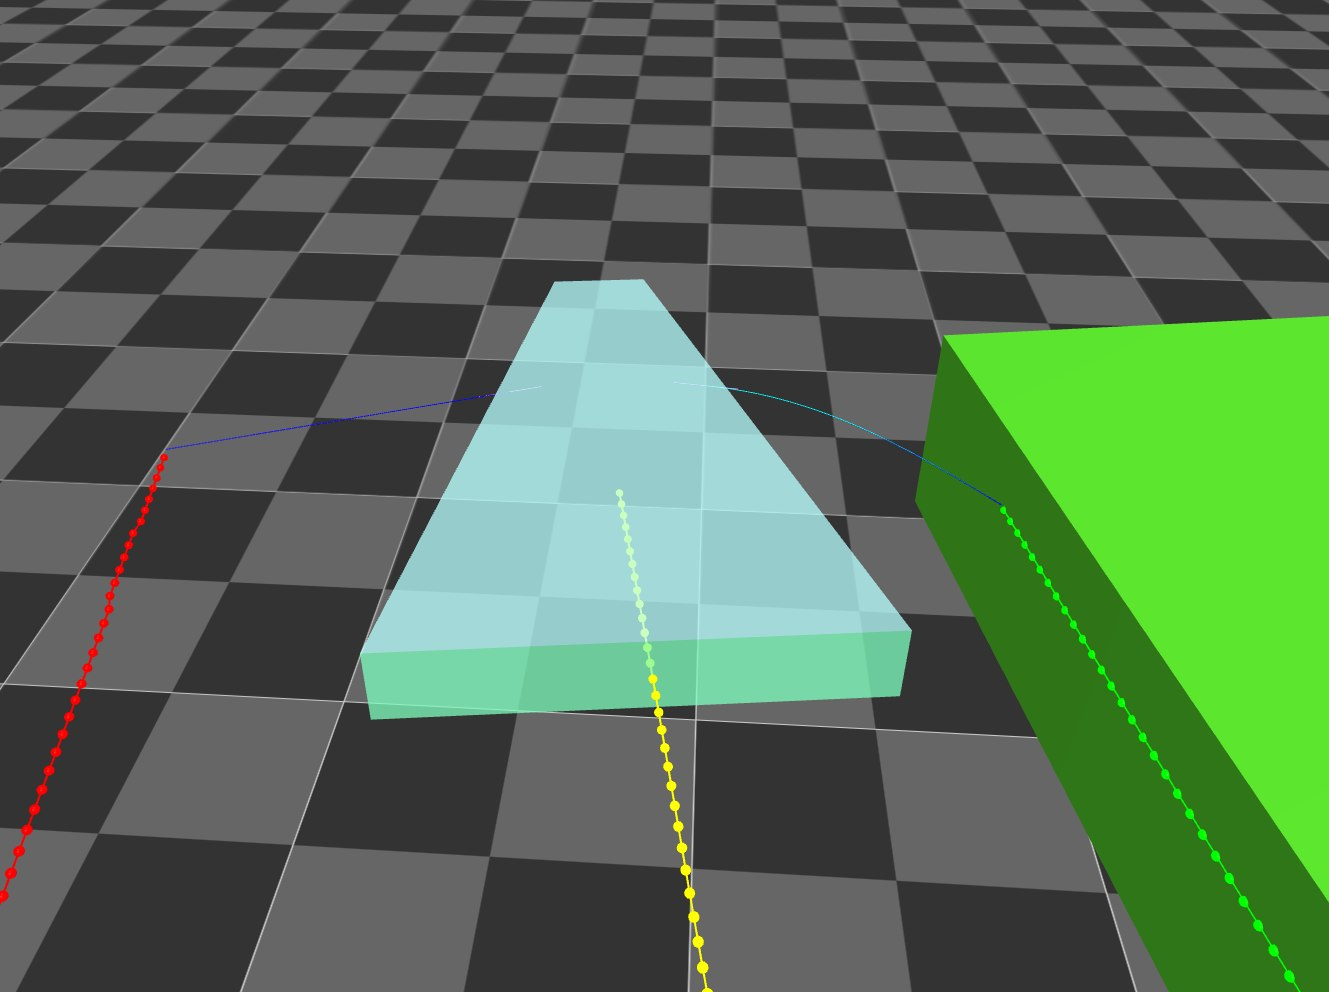
\includegraphics[width=\textwidth]{figures/retrieval/before}
        \caption{\textbf{Initial situation}\\Swiping along the side of the object.}
        \label{fig:retrieval-0-1}
    \end{subfigure}\hfill
    \begin{subfigure}[b]{0.47\textwidth}
        \centering
        \captionsetup{justification=centering}
        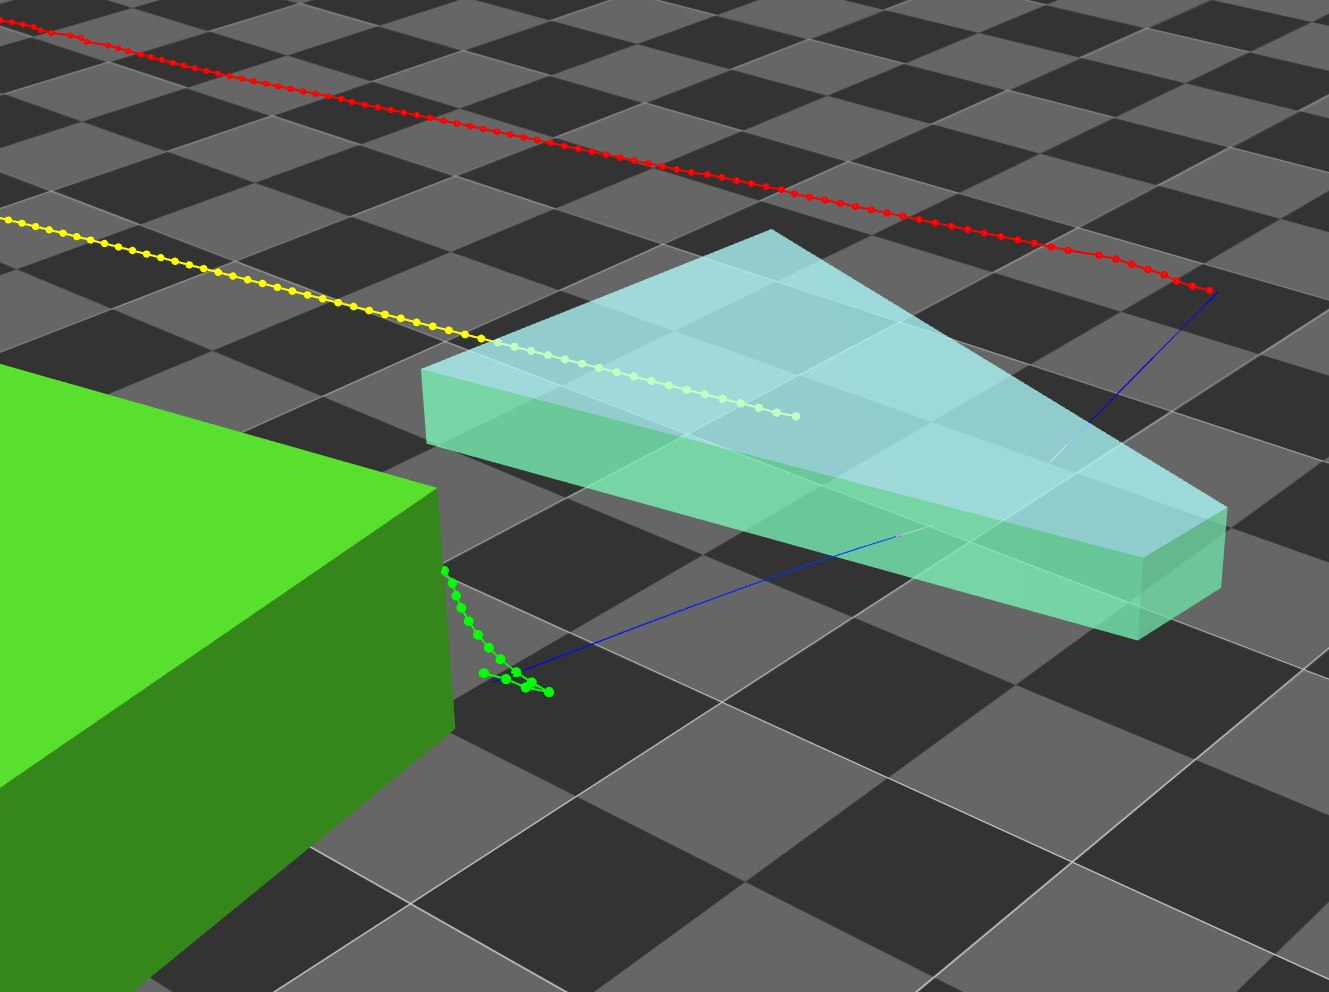
\includegraphics[width=\textwidth]{figures/retrieval/disengagement}
        \caption{\textbf{Disengagement}\\Whisker has detached.}
        \label{fig:retrieval-0-2}
    \end{subfigure}
    \begin{subfigure}[b]{0.47\textwidth}
        \centering
        \captionsetup{justification=centering}
        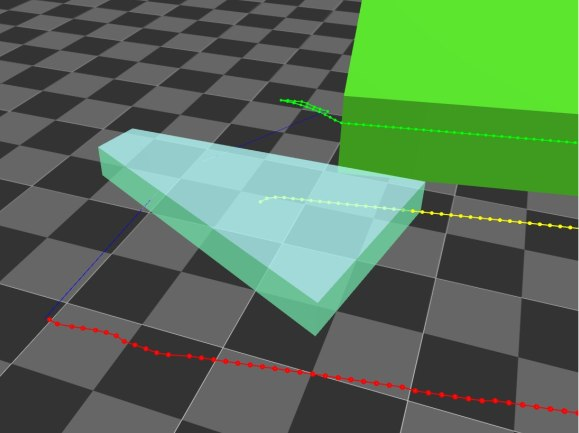
\includegraphics[width=\textwidth]{figures/retrieval/mid-retrieval}
        \caption{\textbf{Rotation}\\Whisker is rotating around the edge.}
        \label{fig:retrieval-1-1}
    \end{subfigure}\hfill
    \begin{subfigure}[b]{0.47\textwidth}
        \centering
        \captionsetup{justification=centering}
        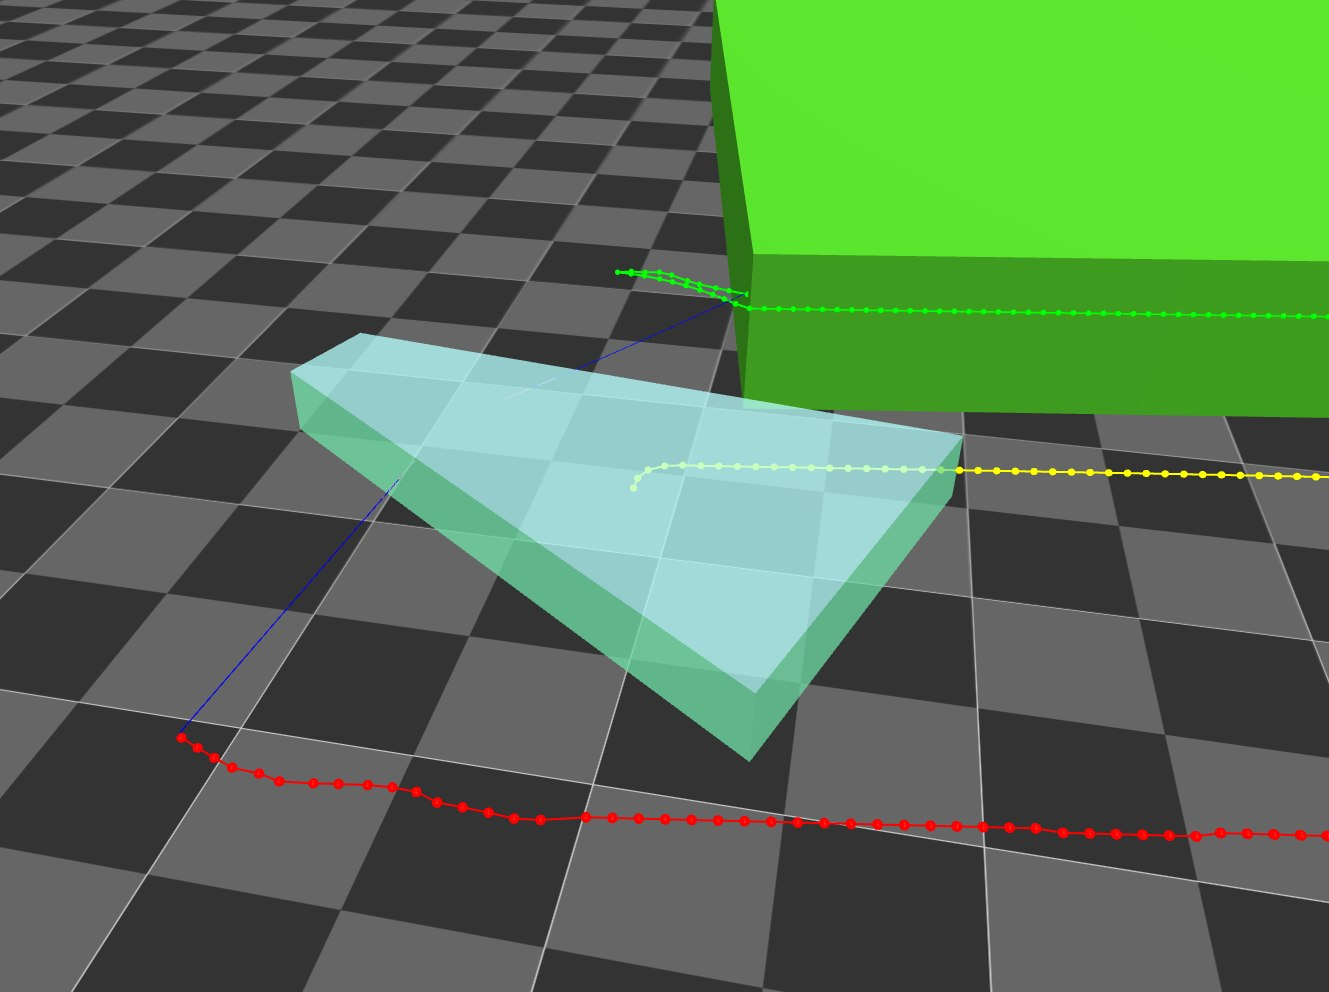
\includegraphics[width=\textwidth]{figures/retrieval/retrieval}
        \caption{\textbf{Retrieval}\\Whisker has retrieved the contact.}
        \label{fig:retrieval-1-2}
    \end{subfigure}
    \begin{subfigure}[b]{0.47\textwidth}
        \centering
        \captionsetup{justification=centering}
        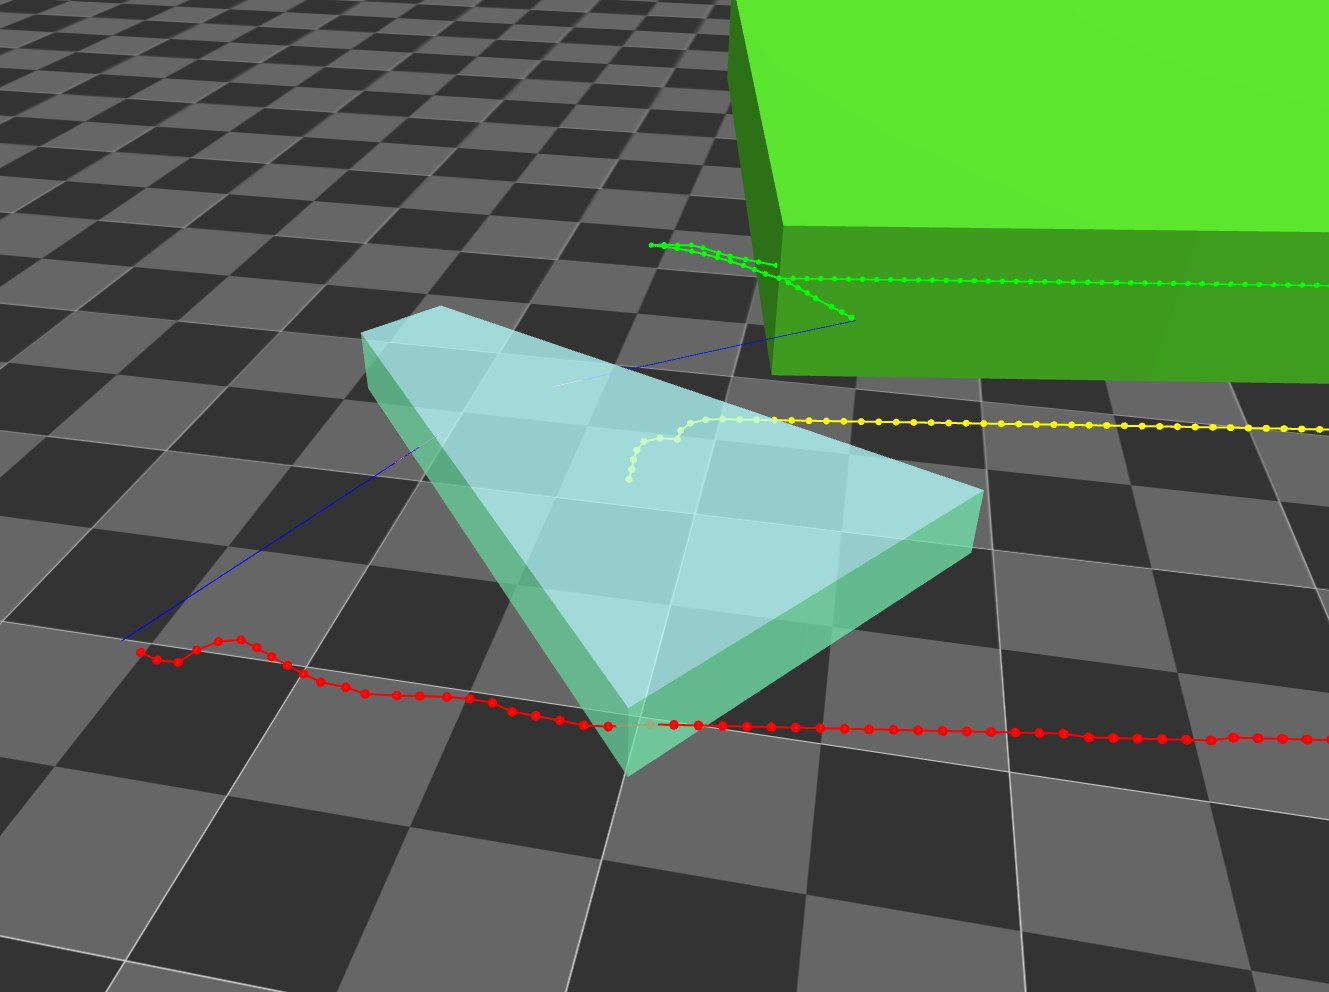
\includegraphics[width=\textwidth]{figures/retrieval/whisking}
        \caption{\textbf{Whisking}\\Moving back along the opposite side of the edge.}
        \label{fig:retrieval-2-1}
    \end{subfigure}\hfill
    \begin{subfigure}[b]{0.47\textwidth}
        \centering
        \captionsetup{justification=centering}
        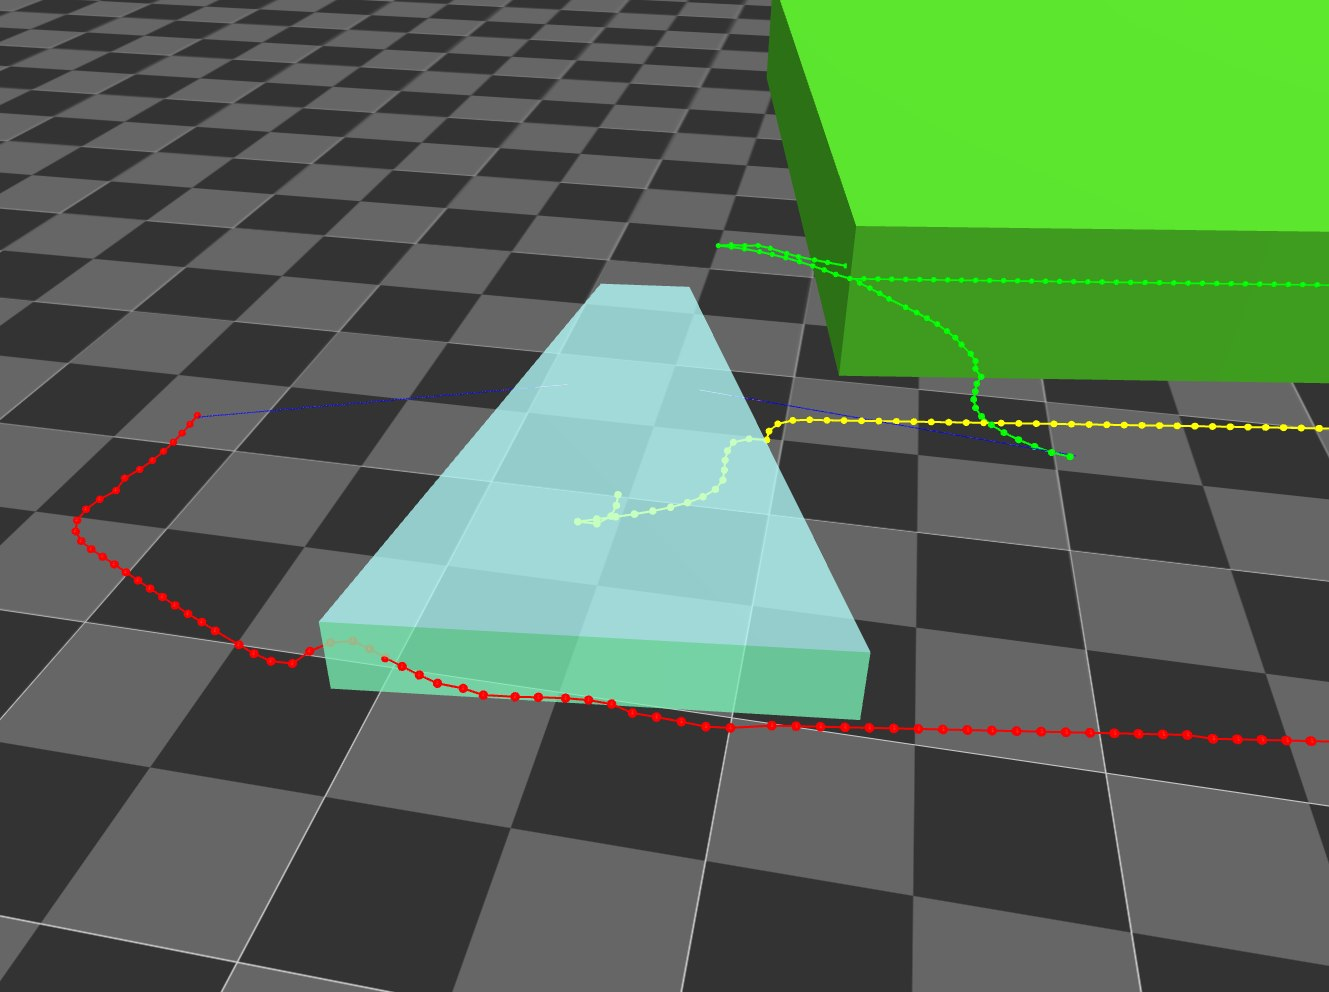
\includegraphics[width=\textwidth]{figures/retrieval/repositioning}
        \caption{\textbf{Repositioning}\\Assuming an optimal position for approach.}
        \label{fig:retrieval-3-1}
    \end{subfigure}
    \begin{subfigure}[b]{0.47\textwidth}
        \centering
        \captionsetup{justification=centering}
        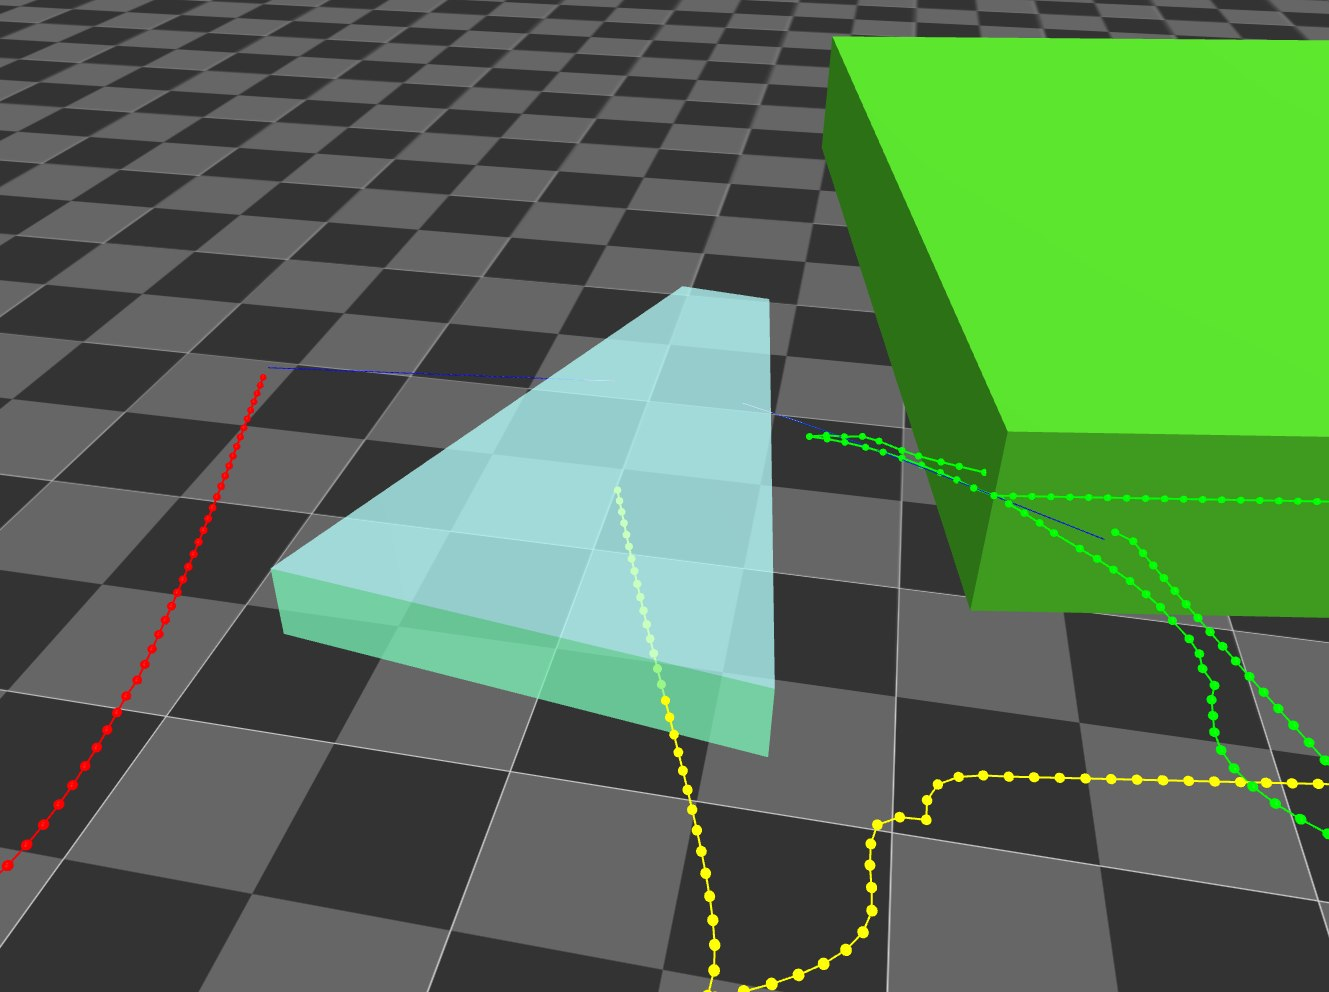
\includegraphics[width=\textwidth]{figures/retrieval/approach}
        \caption{\textbf{Approach}\\Moving towards the object.}
        \label{fig:retrieval-3-2}
    \end{subfigure}\hfill
    \begin{subfigure}[b]{0.47\textwidth}
        \centering
        \captionsetup{justification=centering}
        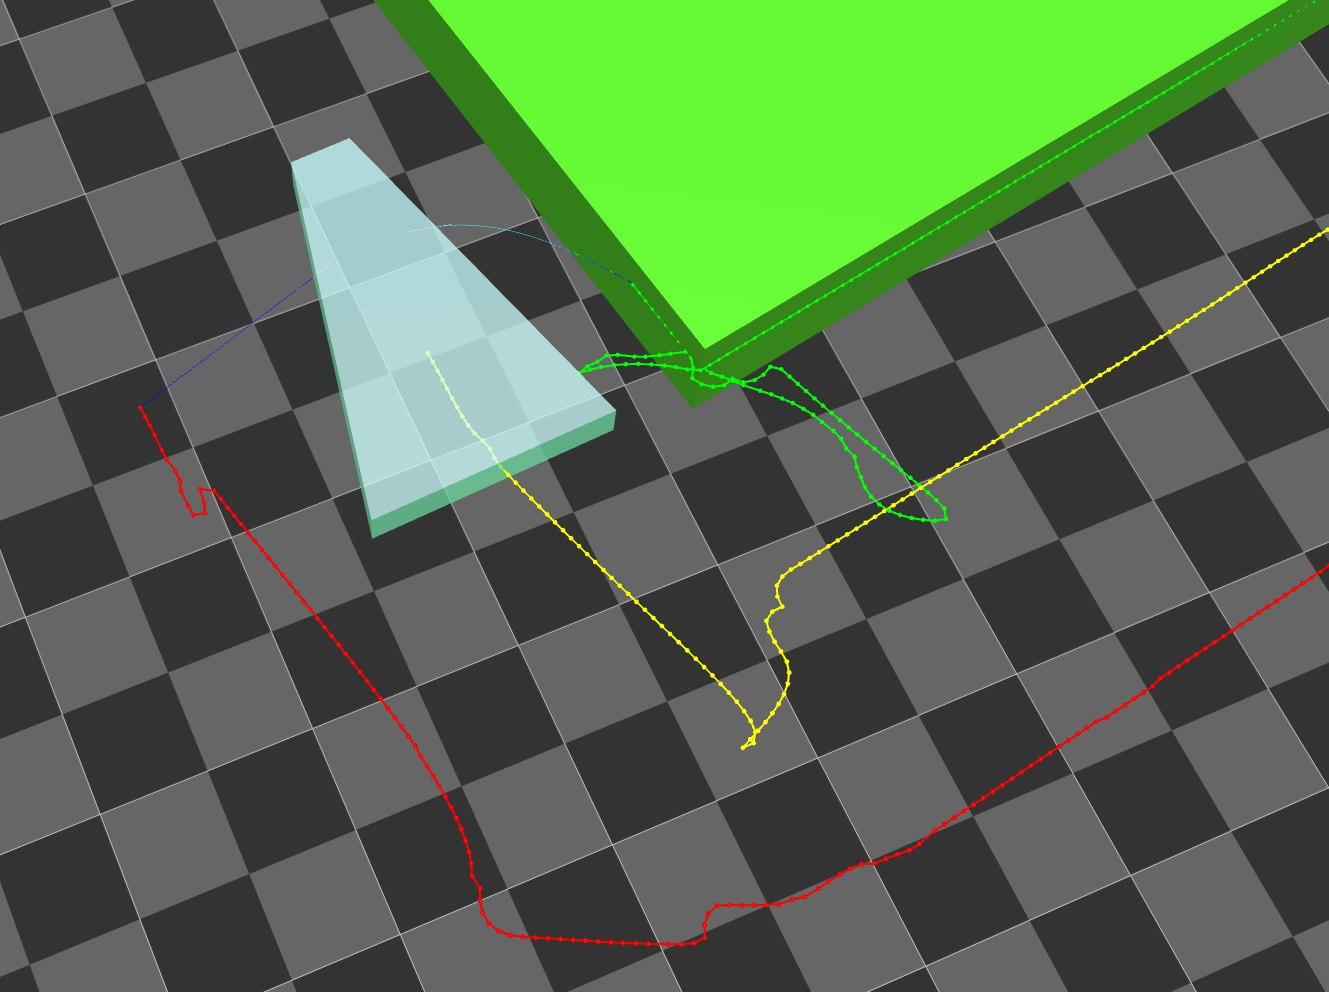
\includegraphics[width=\textwidth]{figures/retrieval/trajectory}
        \caption{\textbf{Transition to Swiping}\\Transferring control to the Swiping Policy.}
        \label{fig:retrieval-3-3}
    \end{subfigure}
    \caption{Retrieval Policy in 8 steps.}
    \label{fig:retrieval}
\end{figure}


\section{Tunneling Policy}

The tunneling policy ensures that the platform maintains a centered trajectory between two surfaces, which optimizes whisker contact on both sides.
The idea is demonstrated in Algorithm~\ref{alg:tunneling_policy}.
A midpoint spline is generated by computing keypoints defined as the midpoints between the left and right whisker contacts (Algorithm~\ref{alg:tunneling_policy}, lines 1--3 highlighted in yellow).
This B-Spline is a continuous reference for steering the platform through tunnel-like environments.
The target angle is determined by the tangent of the midpoint spline (Algorithm~\ref{alg:tunneling_policy}, lines 6--8 highlighted in blue).
The target position is calculated as the current position plus the weighted sum of the spline tangent and deflection \enquote{pull} (Algorithm~\ref{alg:tunneling_policy}, lines 9--10 highlighted in green).
This pull evaluates the difference between the current and target deflections as a ratio for both whiskers and shows whether normal movement is needed to correct the deflection.

\begin{algorithm}
    \caption{Tunneling Policy}
    \begin{algorithmic}[1]
        \State \colorbox{yellow!40}{\(\;^{\mathrm{w}}\boldsymbol{r}_{\mathrm{tip, r}}^{t} \gets \;^{\mathrm{w}}\boldsymbol{r}^{t} + \;^{\mathrm{w}}\boldsymbol{r}_{\mathrm{r, body}} + \boldsymbol{R}_{xy}^{2}(\; ^{\mathrm{w}}\alpha_{\mathrm{r}}^{t}) \cdot \mathrm{r.defl\_model}(\delta_{\mathrm{r}}^{t})\)}
        \State \colorbox{yellow!40}{\(\;^{\mathrm{w}}\boldsymbol{r}_{\mathrm{tip, l}}^{t} \gets \;^{\mathrm{w}}\boldsymbol{r}^{t} + \;^{\mathrm{w}}\boldsymbol{r}_{\mathrm{l, body}} + \boldsymbol{R}_{xy}^{2}(\; ^{\mathrm{w}}\alpha_{\mathrm{l}}^{t}) \cdot \mathrm{l.defl\_model}(\delta_{\mathrm{l}}^{t})\)}
        \State \colorbox{yellow!40}{\(\mathrm{midpoint\_spline.add\_keypoint}\big((\;^{\mathrm{w}}\boldsymbol{r}_{\mathrm{tip, r}}^{t} + \;^{\mathrm{w}}\boldsymbol{r}_{\mathrm{tip, l}}^{t}) / 2\big)\)}
        \State If not \(\mathrm{midpoint\_spline.has\_enough\_points}\) Then Return \(\;^{\mathrm{w}}\boldsymbol{v}^{t}\), \(\;^{\mathrm{w}}\omega^{t}\) End If
        \State
        \State \colorbox{cyan!40}{\(\;^{\mathrm{w}}\boldsymbol{\tau}_{\mathrm{spline}}^{t} \gets \mathrm{midpoint\_spline}(u\mathord{=}1) - \mathrm{midpoint\_spline}(u\mathord{=}0)\)}
        \State \colorbox{cyan!40}{\(\;^{\mathrm{w}}\boldsymbol{n}_{\mathrm{spline}}^{t} \gets \boldsymbol{R}_{xy}^{2}(\pi/2 \cdot orient_\mathrm{r}^t)\cdot\;^{\mathrm{w}}\boldsymbol{\tau}_{\mathrm{spline}}^{t}\)}
        \State \colorbox{cyan!40}{\(\;^{\mathrm{w}}\theta_{\mathrm{spline}}^{t} \gets \mathrm{arctan2}(\;^{\mathrm{w}}\boldsymbol{\tau}_{\mathrm{spline}}^{t})\)}
        \State \colorbox{green!40}{\(\mathrm{pull_{total}} \gets \mathrm{clip}\big(\frac{\delta_{\mathrm{r}}^{t} - \delta_{\mathrm{r, target}}}{\delta_{\mathrm{r, target}}} - \frac{\delta_{\mathrm{l}}^{t} - \delta_{\mathrm{l, target}}}{\delta_{\mathrm{l, target}}},\mathrm{\min}\mathord{=}-1, \mathrm{\max}\mathord{=}1\big)\)}
        \State \colorbox{green!40}{\(\;^{\mathrm{w}}\boldsymbol{r}^{t+1} \gets \;^{\mathrm{w}}\boldsymbol{r}^{t} + \;^{\mathrm{w}}\boldsymbol{\tau}_{\mathrm{spline}}^{t} + \mathrm{pull_{total}}/2 \cdot \;^{\mathrm{w}}\boldsymbol{n}_{\mathrm{spline}}^{t}\)}
        \State \((\;^{\mathrm{w}}\boldsymbol{v}^{t+1}, \;^{\mathrm{w}}\omega^{t+1}) \gets steer\_body(\;^{\mathrm{w}}\boldsymbol{r}^{t+1},\;^{\mathrm{w}}\theta_{\mathrm{spline}}^{t})\)
        \State Return \(\;^{\mathrm{w}}\boldsymbol{v}^{t+1}, \;^{\mathrm{w}}\omega^{t+1}\)
    \end{algorithmic}
    \label{alg:tunneling_policy}
\end{algorithm}


\section{Finite State Machine}

The policies are specialized, and only in combination can the whisker harness their full potential.
An FSM combines these policies, with each policy represented as a state.
Transitions occur when specific events arise, such as ``whisker has come into contact with the surface'' or ``whisker has become disengaged.''
The state chart of the FSM for the discussed policies is depicted in Figure~\ref{fig:fsm}.

\begin{figure}[htb]
    \centering
    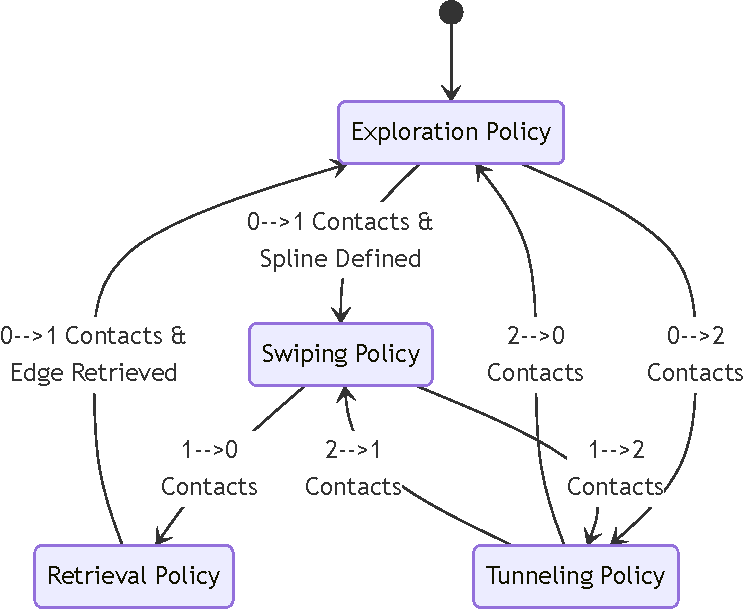
\includegraphics[width=0.8\textwidth]{figures/diagrams/fsm}
    \caption{FSM diagram of the whisker control system. The diagram illustrates the various states (Exploring, Swiping, Tunneling, Retrieval, Whisking, Failure) and the transitions triggered by contact establishment, detachment, and reattachment.}
    \label{fig:fsm}
\end{figure}


\section{Additional features}

Additional modifications can be applied to the control algorithm depending on the specific requirements of the task.

\subsection{Retrieval without Edge Reconstruction}

If the goal is to quickly analyze the object's surface without precise edge reconstruction, the whisking step in the retrieval policy can be skipped so that the angle resolution stage directly leads to swiping on the opposite side.

\subsection{Platform Tilt}

The platform can be tilted slightly toward the object for improved stability during swiping (i.e., to handle sharper angles without separation).
This requires a simple modification of the body motion control algorithm by adjusting the target orientation by a small angle.
The tilt increases the duration of whisker contact with the surface as the platform maintains its direction.
It is beneficial given that the spline is constructed only at the contact point and cannot predict the future curve far away.

\subsection{Reverse Swiping}

If it is necessary for the platform to backtrack its path, the swiping policy can be modified to follow the spline in the reverse direction.
This is achieved by redefining the principal movement direction (normally aligned with the \enquote{nose} of the platform) in reverse mode.
Consequently, the body motion control algorithm computes the linear velocity using an oppositely offset yaw.
The retrieval policy is adjusted accordingly, as it depends solely on the position of the whisker base and is independent of the platform's overall orientation.

\subsection{Positioning of Whiskers at Different Angles}

Improving the adhesion of the whisker to the object can be achieved by positioning the whisker at an angle relative to the platform while maintaining the platform's tangential alignment with the object.
This approach follows the same principle as tilting but preserves the platform's angle relative to the object.
This modification is particularly important in tunneling scenarios, where both whiskers must negotiate turns without becoming stuck.
When entering a tunnel, the first whisker contacts the surface, followed by the second whisker.
It is critical that the second whisker is positioned at an appropriate angle relative to the platform (typically slightly behind the main body).
If the whisker points directly in the direction of movement, it may insert into surface cavities and bend as if the platform were moving in the opposite direction, risking damage due to excessive deflection.
Positioning the whisker slightly backward prevents direct head-on contact with the tunnel wall.

\subsection{Integration of Multiple Whiskers on Each Side}

Multiple whiskers can be integrated on each side of the platform to:
\begin{itemize}
    \item Increase the precision of surface resolution.
    \item Enable single-shot swiping without the need for retrieval, as the retrieval radius is smaller than the distance between two whisker bases.
    \item Detect contacts at a wider range by extending the search space.
\end{itemize}


\section{Comparison to the Baseline}

The control algorithm by \textcite{dang2025whisker} is used as a baseline for comparison, as this work directly builds upon it.

\subsection{Baseline Algorithm}

The baseline algorithm from previous work implements the swiping policy as follows:
\begin{enumerate}
    \item A Kalman filter is applied for preprocessing, using measurement noise covariance to estimate the whisker deflection offset.
    \item The swiping policy employs a single PID controller that takes the whisker deflection error as input and returns the desired velocity in the direction of the object (in the sensor frame).
    \item The total velocity is maintained, with the principal direction velocity in the local frame calculated as the complement to the velocity toward whisker compression or relaxation.
    \item The output velocity in the world frame is obtained by rotating the local frame velocity by the whisker tip spline tangent.
\end{enumerate}
The underlying idea is that to track the surface, the whisker deflection profile must remain constant; hence, the platform moves closer to the object when the whisker is too relaxed and moves away when it is too strained.

\subsection{Comparison to Baseline}

The baseline control can be characterized as follows:
\textbf{Pros:}
\begin{itemize}
    \item The whisker deflection offset is less susceptible to noise due to filtering.
    \item The swiping policy is straightforward and is designed to maintain a constant whisker profile.
\end{itemize}

\textbf{Cons:}

\begin{itemize}
    \item Filtering does not resolve the inherent noise or limitations of an ill-posed deflection model; subtle changes in whisker deflection that may be important for surface reconstruction can be lost.
    \item Maintaining a constant deflection profile ensures surface tracking but does not guarantee complete contour capture.
    \item The platform's velocity is relatively slow, and sudden changes in the principal direction--due to whisker slippage--can result in a 180° change in the spline direction, potentially causing reverse motion.
\end{itemize}

The following steps are possible to rectify the shortcomings of the baseline algorithm:
\begin{enumerate}
    \item To enhance reactivity, remove the Kalman filter and apply smoothing directly to the deflection signal (using the low-pass Butterworth filter described in Section~\ref{sec:data_preprocessing}).
    \item To modify the swiping policy to balance the importance of following the spline with maintaining the deflection profile.
    \item To introduce a whisker orientation parameter (clockwise or counterclockwise) to prevent the whisker profile from deflecting in the opposite direction during control.
    This orientation is set upon initial contact with the surface and is preserved until the whisker disengages.
    It is employed in the calculation of the desired whisker base-tip offset.
\end{enumerate}

\subsection{Limitations of the Suggested Control Algorithm}
The proposed control algorithm has several limitations:
\begin{itemize}
    \item It does not consider the platform dimensions to prevent non-whisker contacts.
    \item It requires parameter tuning (e.g., velocity, desired deflection, contact deflection threshold, PID parameters, etc.).
    \item It is not failsafe regarding whisker integrity, as extreme deflections are not directly forbidden.
    \item It does not allow for non-constant velocity and does not optimize the velocity for the environment.
    \item It can lead to situations where the platform might get stuck (for instance, at the tunnel end, since the minimal space required for platform rotation without damaging the whisker is not calculated).
    \item There are other limitations imposed by the assumptions discussed earlier.
\end{itemize}

    % !TeX spellcheck = en_US


\chapter{Experimental Setup}

We developed a simulation framework, tools for collecting metrics, and an automatic test runner to validate the proposed policies.
It is backed by MuJoCo~\cite{todorov2012mujoco}, which provides a realistic simulation of contact dynamics.
Our developed framework is available on GitHub\footnote{\url{https://github.com/SVDouble/RatteChan}}.


\section{Swiping Policy} \label{sec:swiping-policy}

For the swiping policy, a single whisker executes a sweeping motion over the object.
Performance is quantified by evaluating the mean absolute error and the standard error in contour reconstruction, with each estimated point $\mathbf{y}_i$ matched to its closest reference point $\mathbf{x}_i$.

The estimated contour, $C_{\text{est}} = \{\mathbf{y}_i\}_{i=1}^N$, is determined by the control algorithm, which selects points based on whisker deflection and excludes those recorded during the whisking-back phase in retrieval.
The reference contour, $C_{\text{ref}} = \{\mathbf{x}_i\}_{i=1}^N$, consists of points on the object's surface, each being the closest match to the corresponding estimated point, and is derived from high-resolution sampling to serve as ground truth.

The absolute error is $d_i = \|\mathbf{x}_i - \mathbf{y}_i\|$, which is the Euclidean distance between the reference and estimated points.
To assess performance, we compute the mean absolute error
\[
    \bar{d} = \frac{1}{N}\sum_{i=1}^{N} d_i,
\]
and the standard error
\[
    \sigma_d = \sqrt{\frac{1}{N-1}\sum_{i=1}^{N} (d_i - \bar{d})^2}.
\]
The mean absolute error represents the average distance between the reference and estimated points.

Figures~\ref{fig:experiment-disk-swiping}--\ref{fig:experiment-complex-object-swiping} display results for various objects.
Estimated contour points are colored green if their error deviates from the mean by less than the standard error and red otherwise.
Red points indicate the most inaccurate measurements, corresponding to the worst 32 percentile of the error distribution.

Figure~\ref{fig:experiment-disk-swiping} shows the contour estimation of a disk using the swiping policy.
The disk is the simplest object; the mean reconstruction error is $0.8\,\text{mm} \pm 0.5\,\text{mm}$, indicating a high level of accuracy.
No prominent red regions are observed, except for occasional deviations due to the disk's polygonal approximation at the entry point.

\begin{figure}[!htb]
    \centering
    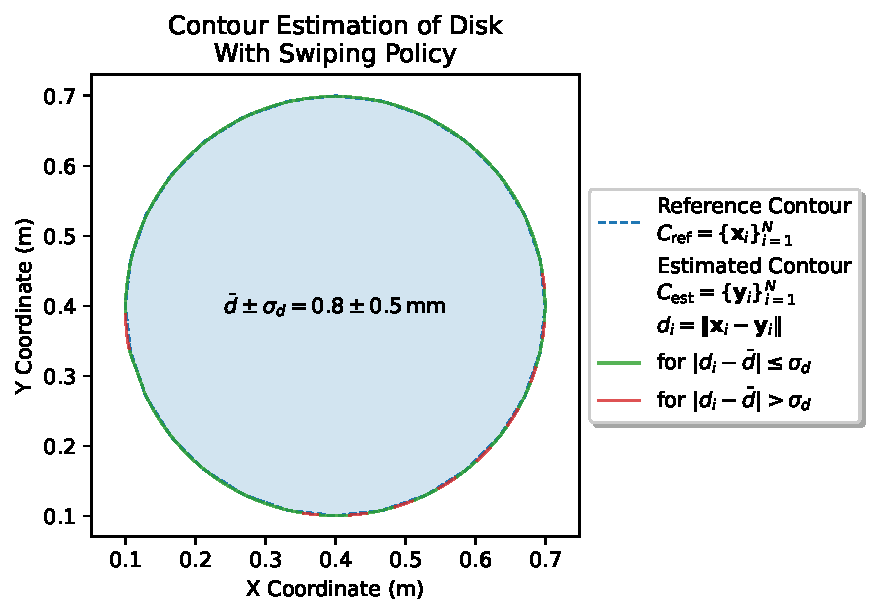
\includegraphics[width=0.8\textwidth]{figures/experiments/disk-swiping}
    \caption{Contour Estimation of Disk With Swiping Policy}
    \label{fig:experiment-disk-swiping}
\end{figure}

Figure~\ref{fig:experiment-rounded-rectangular-box-swiping} illustrates the contour estimation of a rounded rectangular box.
The rounded rectangular box is a more complex object with sharper corners, yet it shows similar accuracy and mean error.
The mean reconstruction error is $0.8\,\text{mm} \pm 0.6\,\text{mm}$, with a single red region after the first corner.

\begin{figure}[!htb]
    \centering
    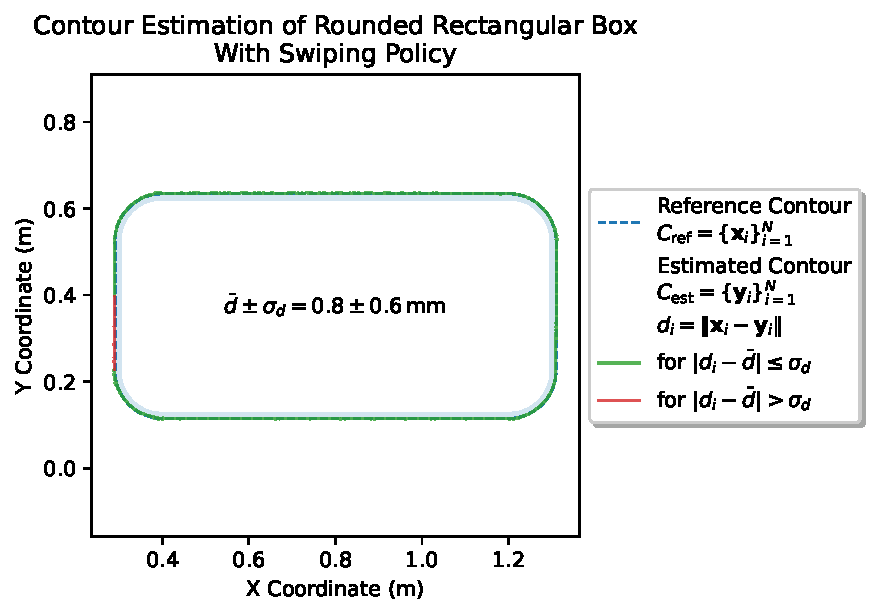
\includegraphics[width=0.8\textwidth]{figures/experiments/rounded-rectangular-box-swiping}
    \caption{Contour Estimation of Rounded Rectangular Box With Swiping Policy}
    \label{fig:experiment-rounded-rectangular-box-swiping}
\end{figure}

Figure~\ref{fig:experiment-complex-object-swiping} shows the contour estimation of a complex object.
Noticeable red regions appear at the inner inflections.
Since the inner angles are not smooth, the platform must quickly adjust to surface changes, which leads to a higher error rate.
At the initial moments, the whisker becomes overly deflected, causing the error to increase as the deflection model performs worse outside its normal operating range.
The mean error remains comparable to that observed for the disk and the rounded rectangular box.

Additionally, the swiping policy can successfully handle a 30\degree{} angle without causing the whisker to detach.
This angle is near the threshold where whisker detachment occurs, and the retrieval policy is triggered.

\begin{figure}[!htb]
    \centering
    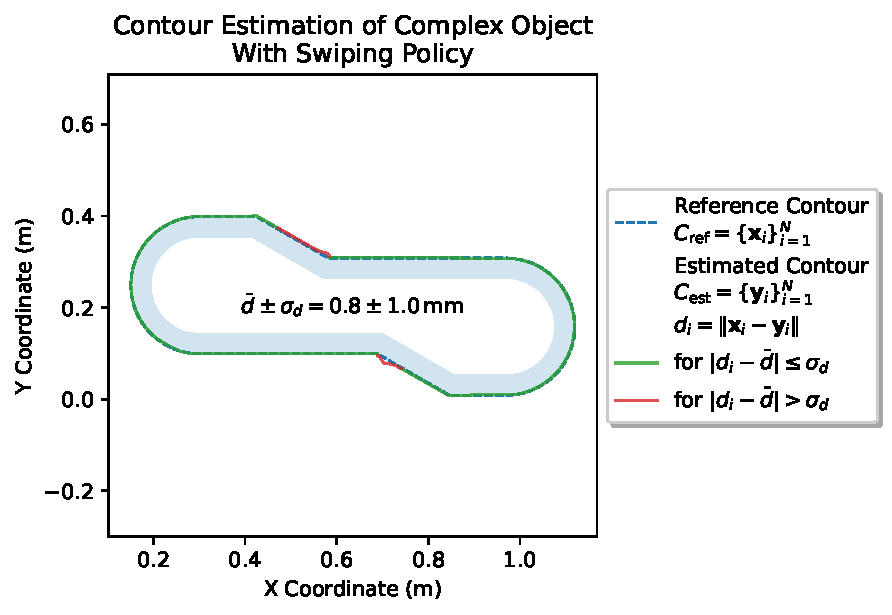
\includegraphics[width=0.8\textwidth]{figures/experiments/complex-object-swiping}
    \caption{Contour Estimation of Complex Object With Swiping Policy}
    \label{fig:experiment-complex-object-swiping}
\end{figure}


\section{Retrieval Policy}

Figures~\ref{fig:experiment-octagon-edges-135deg-swiping-retrieval}--\ref{fig:experiment-wall-edges-90deg-swiping-retrieval} show results for different polygonal objects.
Let $k_{\mathrm{edge}}$ be the index of an edge point and $k_{\mathrm{retr}}$ the index of its corresponding retrieved point, with the same indexing for both events.
The following metrics evaluate the retrieval policy:
\begin{itemize}
    \item \textbf{Mean absolute error:} $\bar{d} = \frac{1}{N}\sum_{i=1}^{N} d_i$, discussed in Section~\ref{sec:swiping-policy}.
    \item \textbf{Mean retrieval radius:} $\bar{r} = \frac{1}{N}\sum_{j=1}^{N} \|\mathbf{r}_{\mathrm{edge},j} - \mathbf{r}_{\mathrm{retr},j}\|$, where $\mathbf{r}_{\mathrm{edge},j}$ is the $j$th edge point and $\mathbf{r}_{\mathrm{retr},j}$ its corresponding retrieved point.
    \item \textbf{Mean retrieval distance:} $\bar{d}_{\mathrm{retr}} = \frac{1}{N}\sum_{j=1}^{N}\sum_{i=i_{\mathrm{edge}_j}}^{i_{\mathrm{retr}_j}-1} \|\mathbf{r}^{t_{i+1}} - \mathbf{r}^{t_i}\|$, which calculates the trajectory length between the time of detachment and the time of retrieval, where $\mathbf{r}^{t}$ denotes the body position at time $t$.
\end{itemize}
In the plots, the edge points $\mathbf{r}_{\mathrm{edge}}$ are shown as red crosses, while the retrieved points $\mathbf{r}_{\mathrm{retr}}$ appear as black crosses.

The mean retrieval radius is defined as
\[
    \bar{r} = \frac{1}{N}\sum_{j=1}^{N} \|\mathbf{r}_{\mathrm{edge},j} - \mathbf{r}_{\mathrm{retr},j}\|,
\]
quantifies the proximity of a retrieved point to the edge, which is critical for accurately determining the edge direction.
A smaller $\bar{r}$ corresponds to a faster and more precise retrieval.
Ideally, this radius should be less than the distance between the whisker tip in its optimally deflected state (with $\delta=\delta_{\mathrm{target}}$) and its neutral state (with $\delta=0$), which is approximately 3\,cm.
The control algorithm sets the target mean retrieval radius to 1\,cm; values below 3\,cm are acceptable, provided the contact angle remains within the desired range.

The mean retrieval distance, given by
\[
    \bar{d}_{\mathrm{retr}} = \frac{1}{N}\sum_{j=1}^{N}\sum_{i=k_{\mathrm{edge},j}}^{k_{\mathrm{retr},j}-1} \|\mathbf{r}^{t_{i+1}} - \mathbf{r}^{t_i}\|,
\]
measures the trajectory length from the time of detachment until the system resumes normal operation after retrieval.
A longer trajectory indicates more unnecessary movement, reducing the efficiency of the retrieval policy.
Note that the whisker's overshoot may increase $\bar{r}$ for large, flat contact angles, even if the backward motion is not required to establish optimal contact.

The retrieval performance for the octagon with 135\degree{} edges is presented in Figure~\ref{fig:experiment-octagon-edges-135deg-swiping-retrieval}.
With its high number of edges, this object demands a stable retrieval policy.
The octagon exhibits a mean reconstruction error of $1.1\,\text{mm} \pm 0.8\,\text{mm}$, comparable to the performance observed with the swiping policy.
It also has a mean retrieval radius of $20.9\,\text{mm} \pm 1.7\,\text{mm}$, about one-quarter of the whisker length.
This radius is higher than the target of 1\,cm because fine adjustment of the whisker's position is unnecessary.
The low relative standard deviation indicates high reproducibility.
The retrieval policy was triggered 8 times in total.

\begin{figure}[!htb]
    \centering
    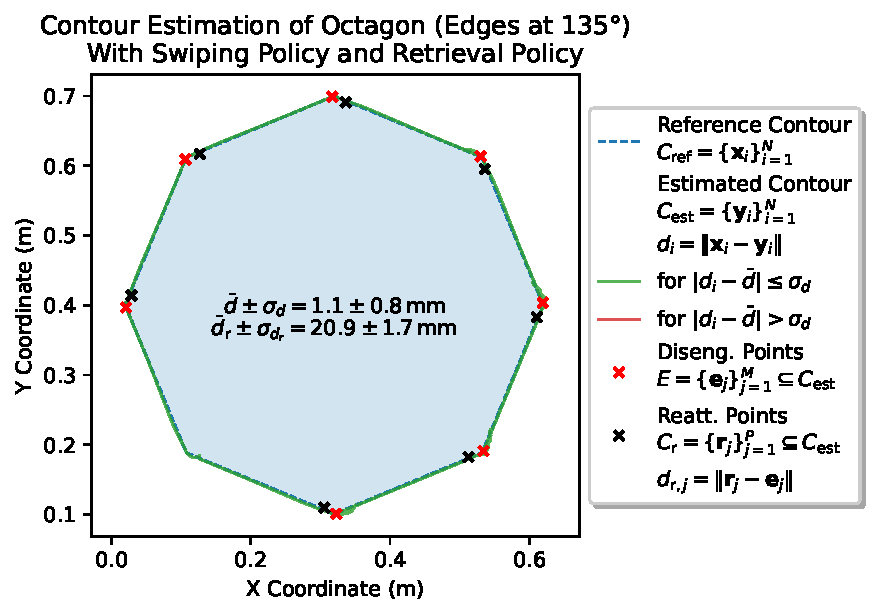
\includegraphics[width=0.8\textwidth]{figures/experiments/octagon-edges-135deg-swiping-retrieval}
    \caption{Contour Estimation of Octagon (Edges at 135\degree{}) With Swiping and Retrieval Policy}
    \label{fig:experiment-octagon-edges-135deg-swiping-retrieval}
\end{figure}

The retrieval on a box with 90\degree{} edges is shown in Figure~\ref{fig:experiment-box-edges-90deg-swiping-retrieval}.
The box's sharper edges present a greater challenge for the whisker.
It achieves a mean reconstruction error of $0.7\,\text{mm} \pm 0.4\,\text{mm}$, demonstrating good performance.
It also has a mean retrieval radius of $11.2\,\text{mm} \pm 1.9\,\text{mm}$, which is close to the 1\,cm target while preserving retrieval consistency.

\begin{figure}[!htb]
    \centering
    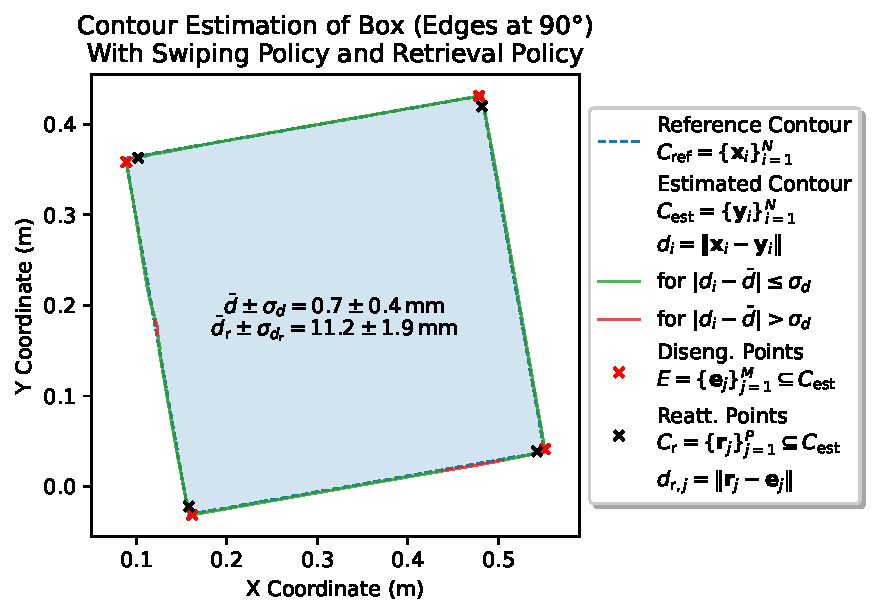
\includegraphics[width=0.8\textwidth]{figures/experiments/box-edges-90deg-swiping-retrieval}
    \caption{Contour Estimation of Box (Edges at 90\degree{}) With Swiping and Retrieval Policy}
    \label{fig:experiment-box-edges-90deg-swiping-retrieval}
\end{figure}

The performance on a prism with 60\degree{} edges is illustrated in Figure~\ref{fig:experiment-prism-edges-60deg-swiping-retrieval}.
The prism yields a mean reconstruction error of $0.8\,\text{mm} \pm 0.6\,\text{mm}$, in line with the swiping policy.
It also has a mean retrieval radius of $8.8\,\text{mm} \pm 0.6\,\text{mm}$, approaching the target value.
However, an inflation in the trajectory is observed at the retrieved edges.
This is likely due to the transition between the undeflected and deflected states.
Such overshooting--especially when the whisker contacts the edge away from its tip--is necessary to accelerate deflection compensation during subsequent swiping.
It also helps minimize the platform's rocking in the normal direction.
A more sophisticated deflection model that accounts for contact along the whisker shaft could potentially mitigate this effect.

\begin{figure}[!htb]
    \centering
    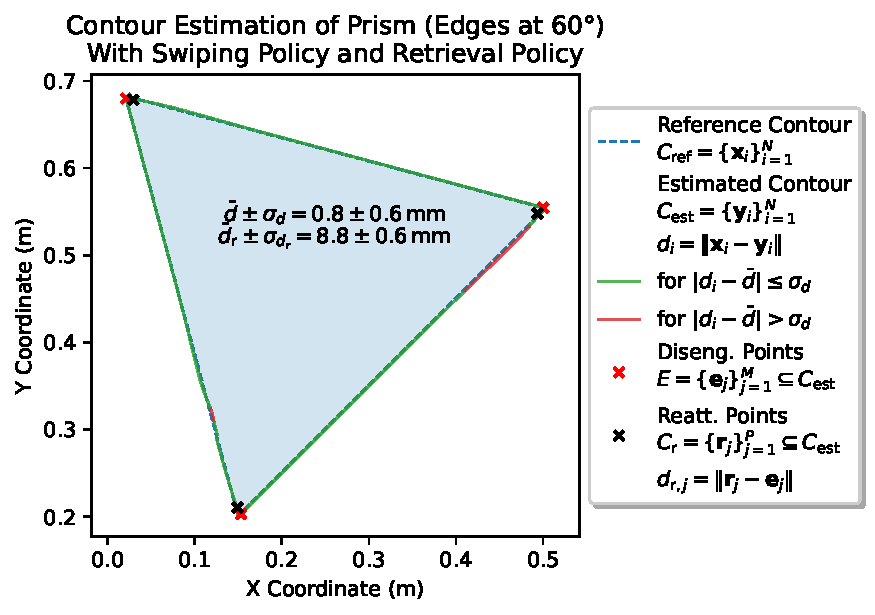
\includegraphics[width=0.8\textwidth]{figures/experiments/prism-edges-60deg-swiping-retrieval}
    \caption{Contour Estimation of Prism (Edges at 60\degree{}) With Swiping and Retrieval Policy}
    \label{fig:experiment-prism-edges-60deg-swiping-retrieval}
\end{figure}

The wall experiment with 90\degree{} edges is presented in Figure~\ref{fig:experiment-wall-edges-90deg-swiping-retrieval}.
This scenario is challenging because the wall's width is only 1\,cm, matching the target retrieval radius.
Nonetheless, the system achieves a mean retrieval radius of $10.2\,\text{mm} \pm 0.7\,\text{mm}$, nearly meeting the target.
This performance is partly due to the wall's precise 1\,cm width, which limits the possibility of contacts farther away.
Video recordings confirm that the whisker tip is well-aligned and contacts the opposite edge accurately.
If the wall were about 25\% shorter, the policy could still handle it through deflection at the whisker's shaft, provided the side length remains above a critical threshold.
Conversely, when the target radius is doubled, the platform executes a 180\degree{} turn to reach the edge, rendering the wall undetectable.
In this case, the mean reconstruction error is $1.1\,\text{mm} \pm 0.6\,\text{mm}$, consistent with the performance of the swiping policy.

\begin{figure}[!htb]
    \centering
    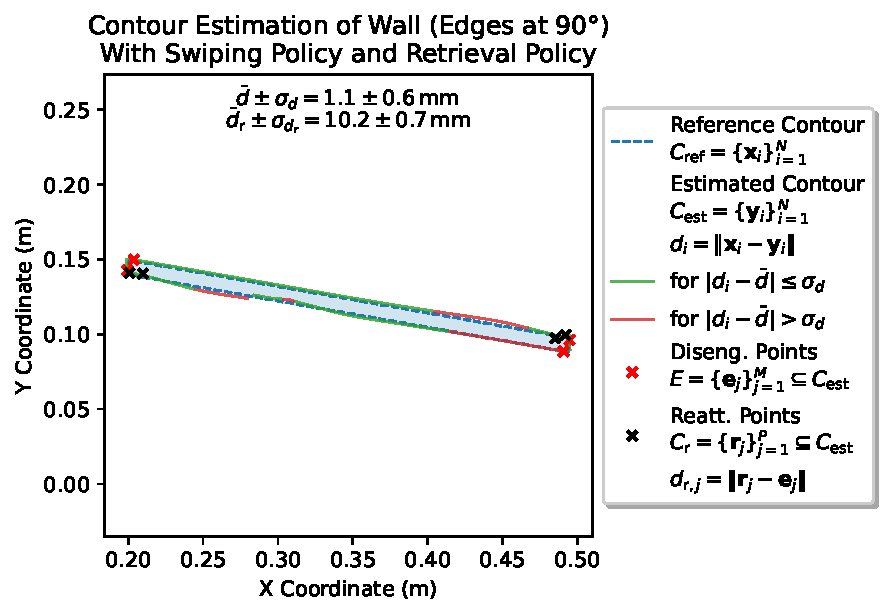
\includegraphics[width=0.8\textwidth]{figures/experiments/wall-edges-90deg-swiping-retrieval}
    \caption{Contour Estimation of Wall (Edges at 90\degree{}) With Swiping and Retrieval Policy}
    \label{fig:experiment-wall-edges-90deg-swiping-retrieval}
\end{figure}


\section{Tunneling Policy}
A tunneling policy extends the swiping policy to navigate confined environments.
Its goal is to maintain a centered trajectory in the tunnel to avoid collisions and ensure accurate contour estimation.

For the tunneling policy, we employ the following metrics:

\begin{itemize}
    \item \textbf{Mean absolute reconstruction error:}
    \[
        \bar{d} = \frac{1}{NK}\sum_{i=1}^{N}\sum_{k=1}^{K} d_{i,k},
    \]
    where
    \[
        d_{i,k} = \|\mathbf{x}_{i,k} - \mathbf{y}_{i,k}\|
    \]
    is the distance between the $i$th reference point $\mathbf{x}_{i,k}$ and the corresponding estimated point $\mathbf{y}_{i,k}$ of the $k$th whisker.
    \item \textbf{Mean absolute axis error:}
    \[
        \bar{d}_{\mathrm{axis}} = \frac{1}{N}\sum_{i=1}^{N} d_{\mathrm{axis},i},
    \]
    where
    \[
        d_{\mathrm{axis},i} = \|\mathbf{a}_i - \mathbf{a}_m\|
    \]
    is the distance between the point $\mathbf{a}_i$ on the tunnel axis closest to the $i$th estimated midpoint and the axis $\mathbf{a}_m$, with the estimated midpoint defined as
    \[
        \mathbf{m}_i = \frac{\mathbf{x}_{i,\mathrm{l}} + \mathbf{y}_{i,\mathrm{r}}}{2}.
    \]
\end{itemize}

The tunnel axis, shown as pink dashed lines in the figures, is defined as the line equidistant from the tunnel walls.
Thus, the mean absolute axis error quantifies the estimated midpoints (marked in black) deviation from the tunnel axis.

Figures~\ref{fig:experiment-smooth-tunnel-swiping-tunneling}--\ref{fig:experiment-round-tunnel-swiping-tunneling} illustrate smooth, zigzag, and round tunnels.

The smooth tunnel in Figure~\ref{fig:experiment-smooth-tunnel-swiping-tunneling} represents the simplest case.
The whisker successfully navigates the tunnel while maintaining a centered trajectory.
The mean absolute reconstruction error is $1.3\,\text{mm} \pm 1.6\,\text{mm}$, and the mean absolute axis error is $4\,\text{mm} \pm 4\,\text{mm}$.
For reference, the tunnel is approximately 10\,cm wide, and each whisker is 7.5\,cm long.
The difference between the reconstruction error and the axis error is due to a lag in the midpoint trajectory relative to the tunnel axis.
This lag occurs because the control system cannot immediately adjust the platform's position owing to its inertia and the continuously changing tunnel direction.
Additionally, heightened deflection near the operational limit of the deflection model and a transition effect when the whiskers first come into contact with the tunnel walls contribute to this error.

\begin{figure}[!htb]
    \centering
    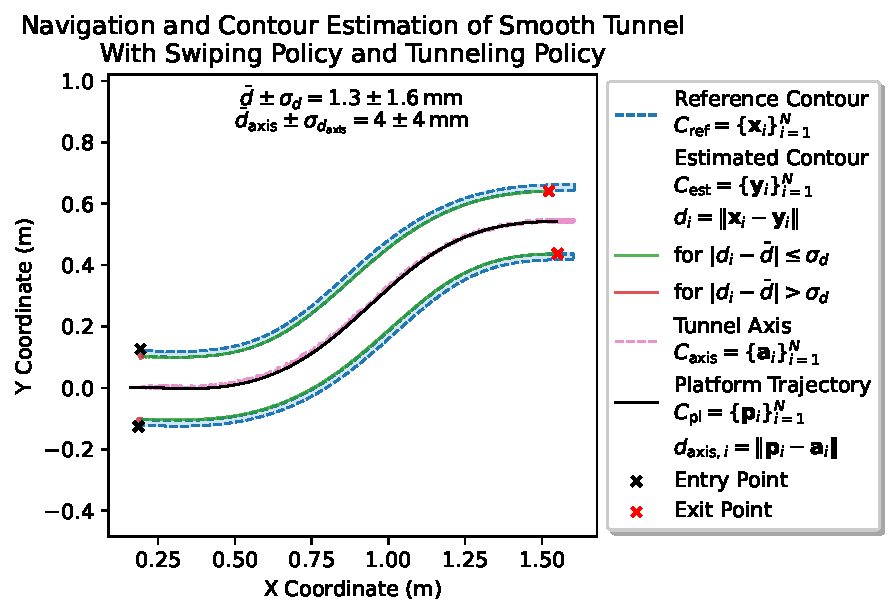
\includegraphics[width=0.8\textwidth]{figures/experiments/smooth-tunnel-swiping-tunneling}
    \caption{Navigation and Contour Estimation of Smooth Tunnel With Swiping and Tunneling Policy}
    \label{fig:experiment-smooth-tunnel-swiping-tunneling}
\end{figure}

The zigzag tunnel in Figure~\ref{fig:experiment-zigzag-tunnel-swiping-tunneling}, with angles of $20^\circ$ and $40^\circ$, is more complex due to its sharper corners.
In this case, the mean absolute reconstruction error is $2\,\text{mm} \pm 2\,\text{mm}$, while the mean absolute axis error increases to $9\,\text{mm} \pm 10\,\text{mm}$.
This increase is attributed to the difficulty of maintaining a centered trajectory, as the midpoint trajectory deviates from the tunnel axis at the corners.
Furthermore, the left whisker detaches at the first zigzag, while the right whisker remains in contact with the wall.
Because the left whisker cannot maintain contact at the sharp angle, the swiping policy is applied to the right whisker until the left whisker re-establishes contact.
The platform's nose contacts the wall for a short period, but it quickly recovers.
Overall, the performance is satisfactory, as the whiskers navigate the tunnel and accurately estimate the contour.
For even sharper zigzag angles, the platform may fail to pass through the tunnel if its nose prods a wall, as no recovery policy is implemented for such cases.
Such failures would be indicated by increased actuator force or a reduced platform speed, which are not measured in the current setup.

\begin{figure}[!htb]
    \centering
    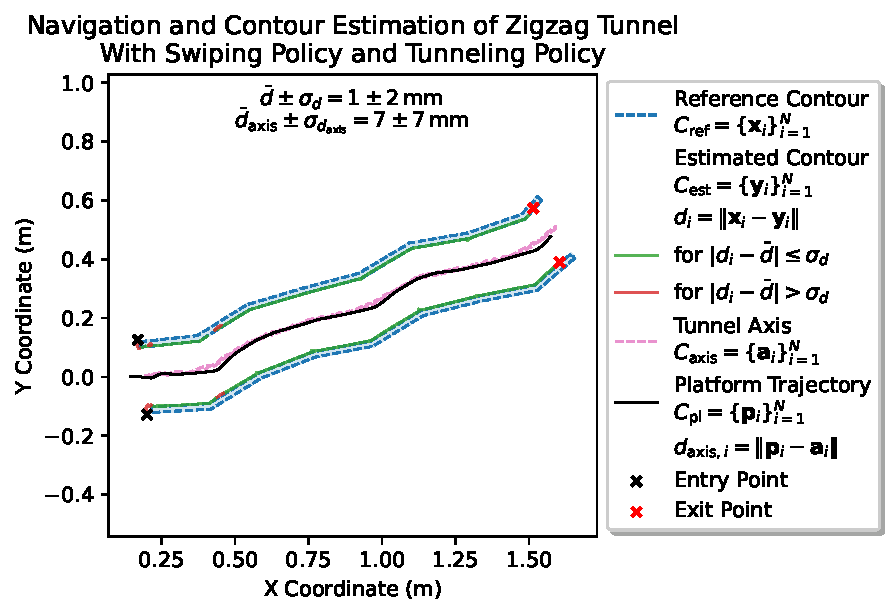
\includegraphics[width=0.8\textwidth]{figures/experiments/zigzag-tunnel-swiping-tunneling}
    \caption{Navigation and Contour Estimation of Zigzag Tunnel With Swiping and Tunneling Policy}
    \label{fig:experiment-zigzag-tunnel-swiping-tunneling}
\end{figure}

The round tunnel in Figure~\ref{fig:experiment-round-tunnel-swiping-tunneling} tests the endurance of the tunneling policy.
It involves a longer trajectory and a star-shaped loop.
A pronounced transition effect is observed at the start, as the whisker adjusts to the tunnel's curvature and the initial position (marked by black crosses) is not aligned with the tunnel axis.
Skidding is also noticeable at the sharper curves.
The performance remains satisfactory, with a mean absolute reconstruction error of $3\,\text{mm} \pm 2\,\text{mm}$ and a mean absolute axis error of $5\,\text{mm} \pm 6\,\text{mm}$.
The increased reconstruction error is likely due to operating outside the optimal range of the deflection model at the curves.
This is evident in segments of the tunnel marked in red, where the outer whisker (right, in this case) experiences excessive compression.

\begin{figure}[!htb]
    \centering
    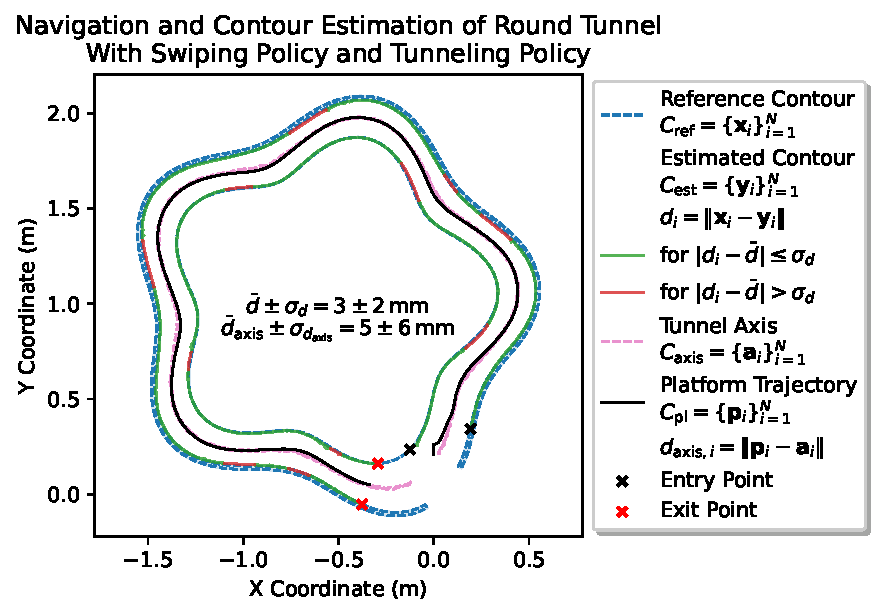
\includegraphics[width=0.8\textwidth]{figures/experiments/round-tunnel-swiping-tunneling}
    \caption{Navigation and Contour Estimation of Round Tunnel With Swiping and Tunneling Policy}
    \label{fig:experiment-round-tunnel-swiping-tunneling}
\end{figure}

    % !TeX spellcheck = en_US


\chapter{Infrastructure}

The following chapter details the integrated system infrastructure that underpins our whisker sensor platform.
It covers the real-time data acquisition, processing, and visualization components and the modular software services orchestrated in Docker containers.
This infrastructure seamlessly connects hardware elements--such as the whisker platform and the actuator--with the control unit and simulation environment.


\section{Overview}
The system infrastructure takes care of real-time sensor data collection, processing, and visualization.
Its implementation is available on GitHub\footnote{\url{https://github.com/SVDouble/RatteChan}} under the \texttt{services} directory.
The architecture comprises three main entities: the whisker platform, the controller, and the actuator.
The platform provides two Inter-Integrated Circuit (I2C) buses for reading sensor data, each equipped with three Adafruit MLX90393 sensors.
The sensors are connected in a daisy chain via a 4-pin JST connector.
This allows us to avoid the need for soldering.
Theoretically, up to 16 sensors can be connected per bus, but we are using only three, as the development boards are limited to four sensors per bus.
The controller device, a Raspberry Pi 5, was chosen because it has sufficient processing power and is small enough to be mounted on the robotic arm.
Currently, the actuator is simulated; however, it will eventually be replaced by a robotic arm.
Figure~\ref{fig:infrastructure_overview} summarizes the system architecture.

\begin{figure}[htb]
    \centering
    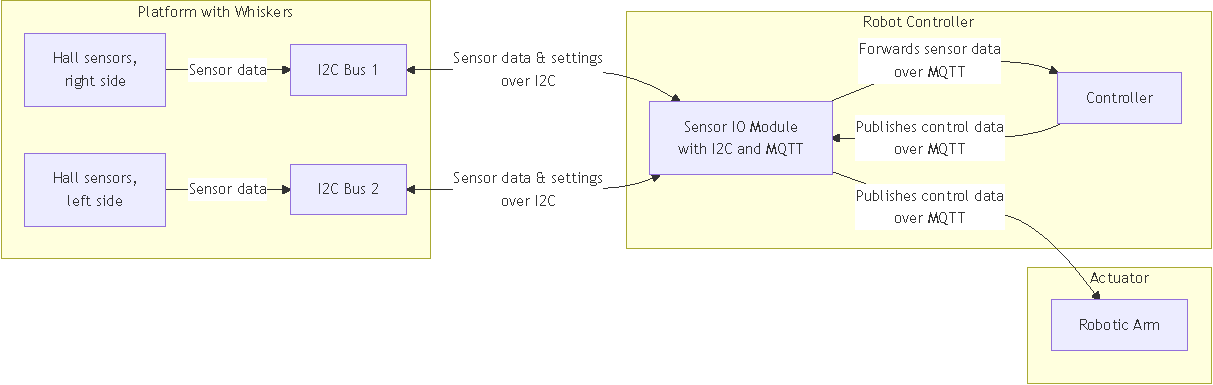
\includegraphics[width=\textwidth]{figures/diagrams/infrastructure-overview}
    \caption{Overview of the system infrastructure.}
    \label{fig:infrastructure_overview}
\end{figure}


\section{Controller}
The control loop of the system is depicted in Figure~\ref{fig:control-flow}.
This loop continuously processes sensor data, evaluates control policies, and generates control messages.
Figure~\ref{fig:control-hierarchy} illustrates the hierarchy of components within the controller.

\begin{figure}
    \centering
    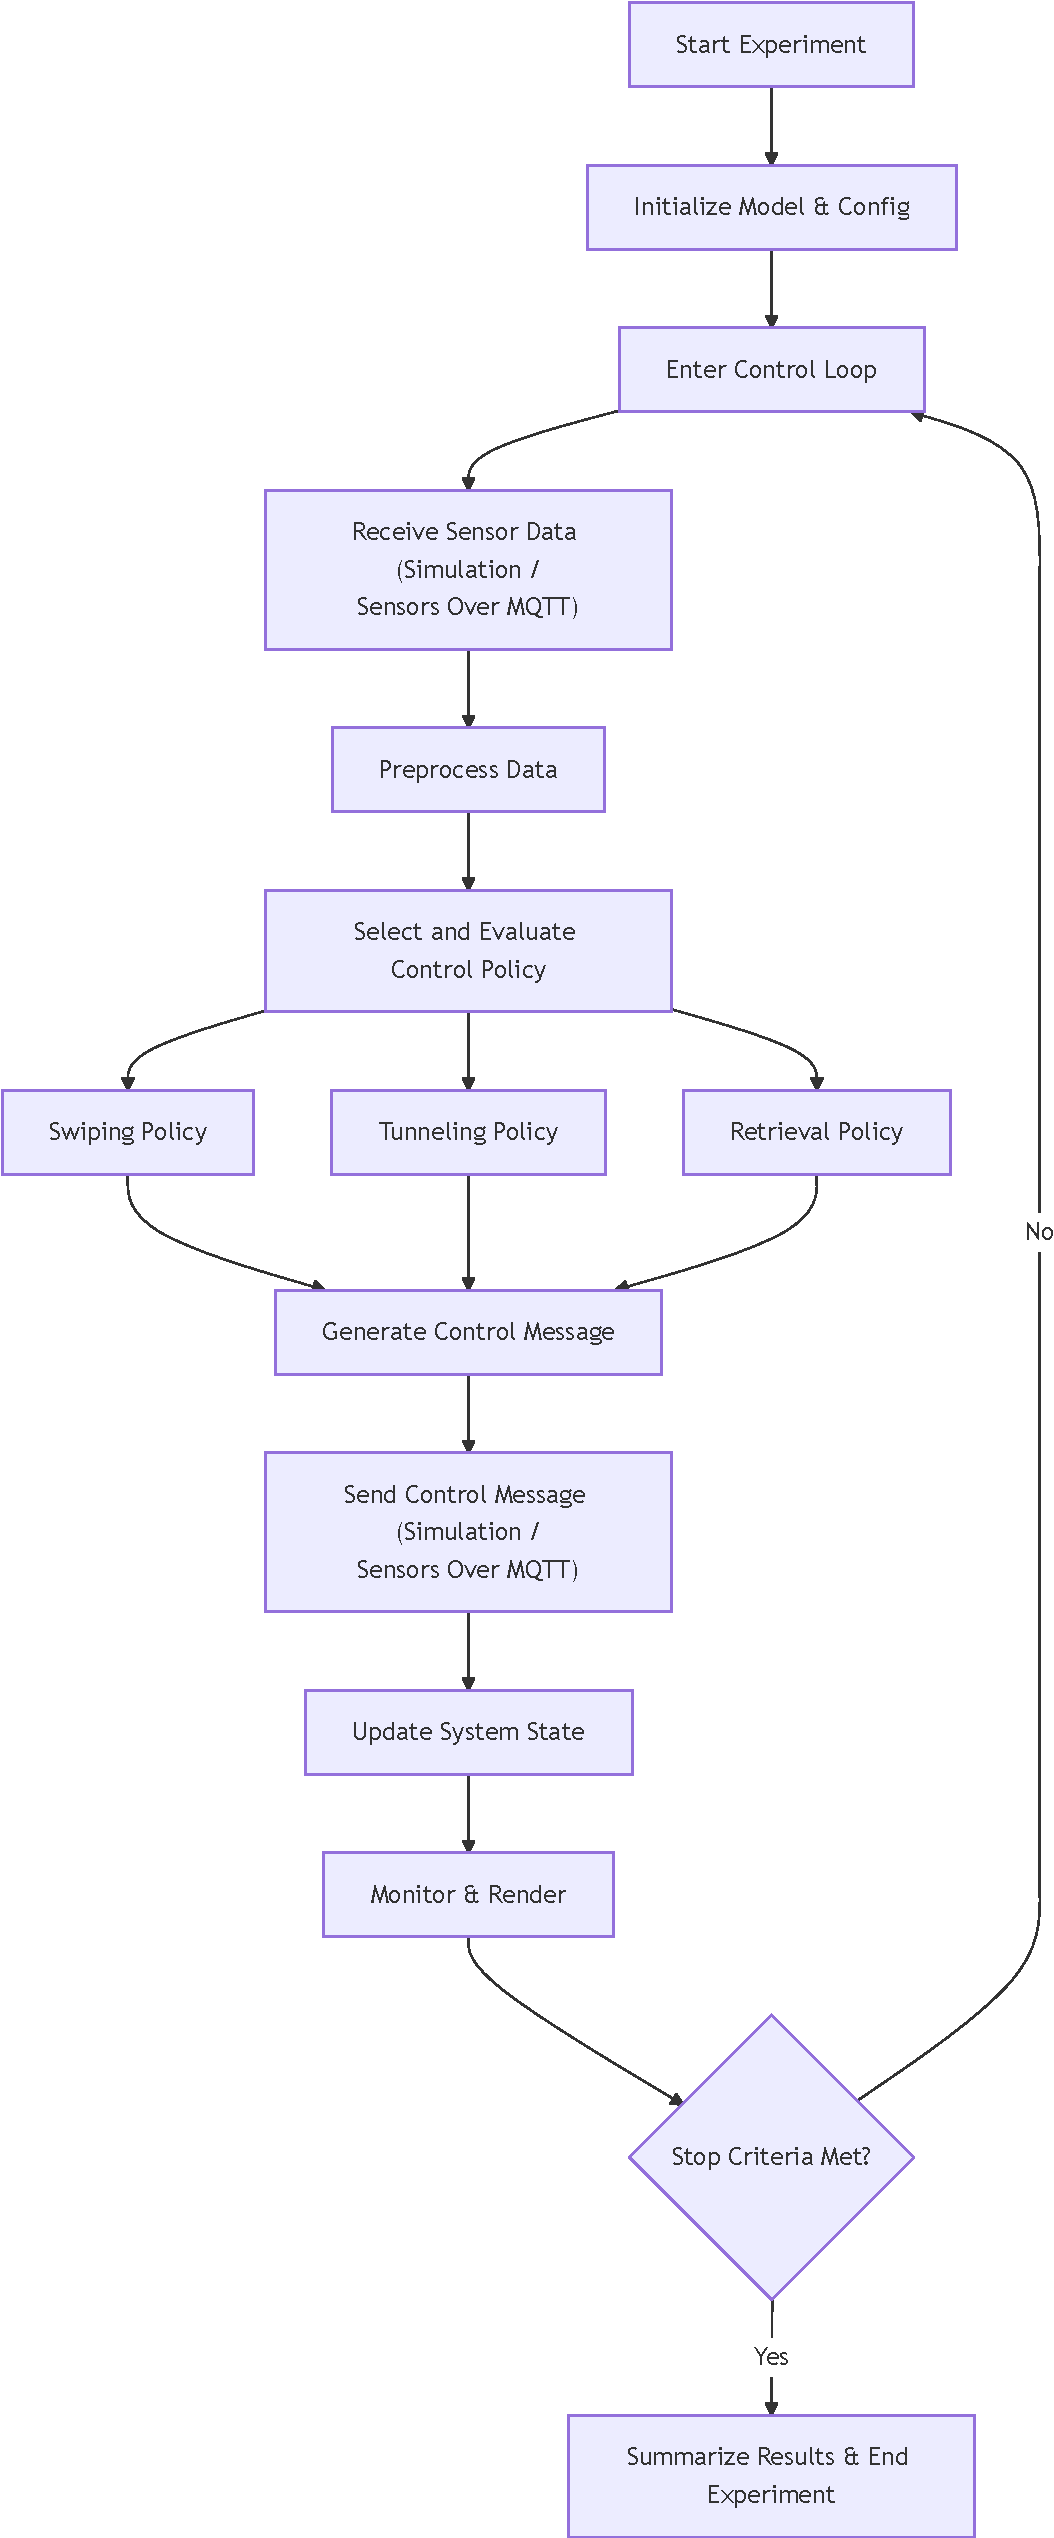
\includegraphics[height=\textheight]{figures/diagrams/control-flow}
    \caption{Data flow in the system infrastructure.}
    \label{fig:control-flow}
\end{figure}


\section{Simulation}
The simulation framework backed by MuJoCo~\cite{todorov2012mujoco} is used for testing the controller.
It provides a realistic environment for validating control algorithms.
Figure~\ref{fig:mujoco} depicts the simulation interface of MuJoCo.

\begin{figure}
    \centering
    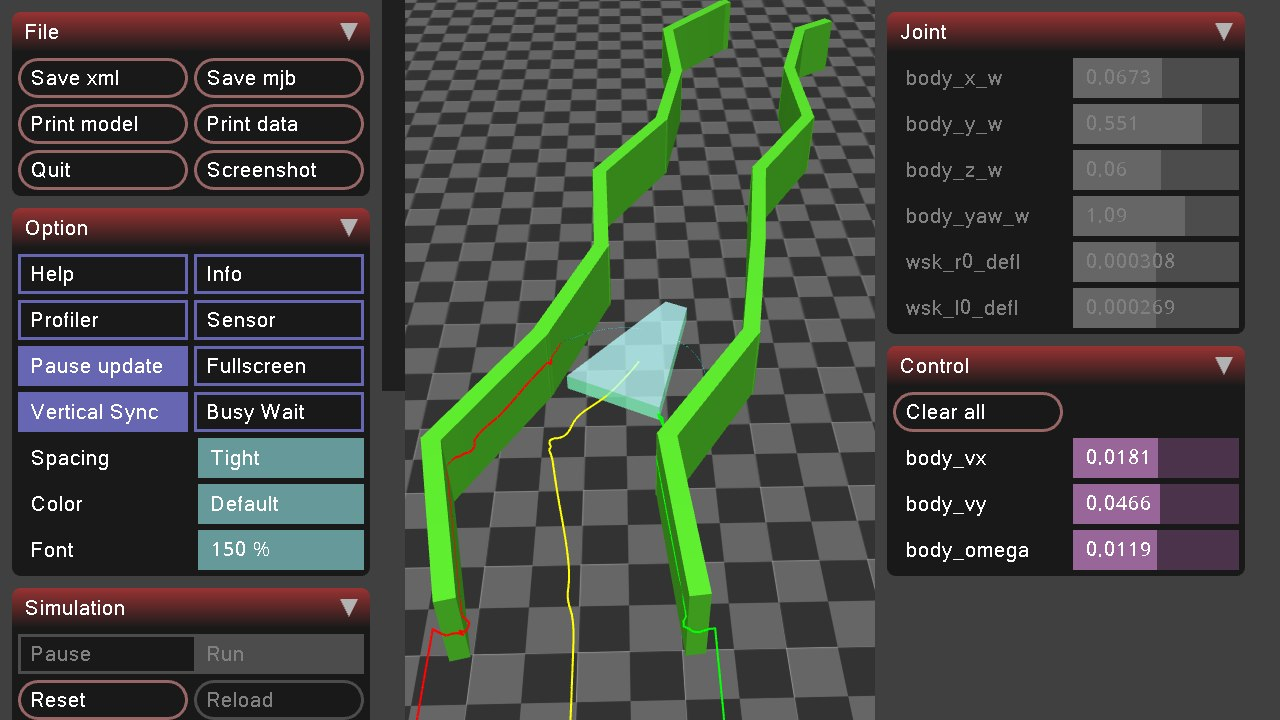
\includegraphics[width=\textwidth]{figures/mujoco}
    \caption{Simulation interface of the MuJoCo physics engine.}
    \label{fig:mujoco}
\end{figure}

The simulation framework is designed to be modular, so the controller has no dependency on the simulation framework.
That makes the integration of new frameworks or sensor data sources and sinks possible.
Ten test cases are provided to test the performance of 3 different policies.
The results are automatically evaluated and plotted for each test case, similar to Figures~\ref{fig:experiment-disk-swiping}--\ref{fig:experiment-round-tunnel-swiping-tunneling}.
An accompanying video is provided for each test case, showing the simulation in action.
MuJoCo allows us to follow, pause, and analyze the simulation.
The simulation is set up so that the trajectories of the whisker tips and the platform center of mass are displayed continuously.
This is a sanity check for the simulation, as the deflection model and tip calculations are error-prone.


\section{System Services}
The system comprises several interconnected services, as illustrated in Figure~\ref{fig:data_flow}.
All of them run in Docker containers to guarantee a consistent and separate environment across different machines.
Docker containers are lightweight, portable, and self-sufficient units that encapsulate all the necessary components to run a software application.
They are orchestrated using Docker Compose\footnote{\url{https://docs.docker.com/compose/}}, a tool for defining and running multi-container applications.
The control system runs on any machine with Docker installed, like Raspberry Pi 5, making it easy to deploy.

\begin{figure}
    \centering
    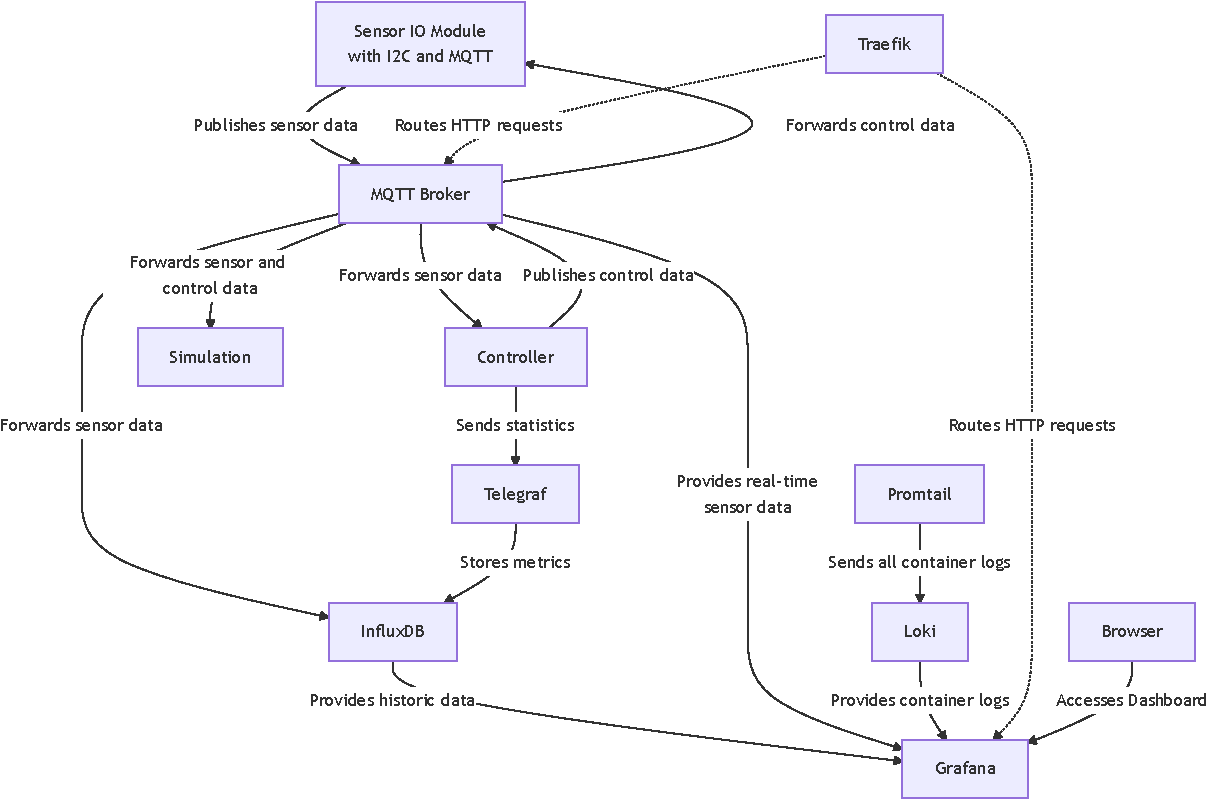
\includegraphics[width=\textwidth]{figures/diagrams/infrastructure-robot-controller}
    \caption{Data flow in the system infrastructure.}
    \label{fig:data_flow}
\end{figure}

\begin{itemize}
    \item \textbf{Sensor IO Module:}
    This module reads sensor data from the robot's I2C buses and publishes the data via Message Queuing Telemetry Transport (MQTT).
    It also forwards control commands from the controller to the actuator.
    Currently, the built-in I2C buses of the Raspberry Pi are used for simplicity.
    But generally speaking, the Sensor IO module can be decoupled from the controller and run on a separate device.

    \item \textbf{Controller:}
    The controller processes sensor data and generates control signals.
    It also publishes statistics for further monitoring.

    \item \textbf{MQTT Broker:}
    As the central messaging hub, the MQTT Broker receives and distributes sensor and control data.
    It is based on the subscriber-publisher model.
    This component is critical for system responsiveness.

    \item \textbf{Telegraf:}
    Telegraf collects sensor data and controller performance metrics.
    The data is then forwarded to InfluxDB for storage.

    \item \textbf{InfluxDB:}
    InfluxDB is a time-series database that stores historical sensor data and controller performance metrics.
    It serves as a persistent storage solution for the system during the execution of the experiments.

    \item \textbf{Grafana:}
    Grafana provides a web-based dashboard that visualizes the sensor data in real time.
    It allows users to monitor the system's status interactively.

    \item \textbf{Promtail:}
    Promtail collects logs from the various services and forwards them to Loki.

    \item \textbf{Loki:}
    Loki aggregates the logs provided by Promtail and makes them available for visualization via Grafana.
    This centralized logging system helps troubleshoot and monitor system health.

    \item \textbf{Traefik:}
    Traefik is a reverse proxy for communication between the services and the outside world.
    For instance, it allows access to the Grafana dashboard via a web browser.
\end{itemize}


\section{Dashboard}
The system dashboard uses Grafana, a powerful analytics and monitoring platform.
It provides a web-based interface for visualizing sensor data and control signals.
Grafana Live with MQTT is employed to transmit real-time system status.
Figure~\ref{fig:grafana} shows a minimalistic dashboard with magnetic data from six whisker sensors sampled in real time.


\begin{figure}[htb]
    \centering
    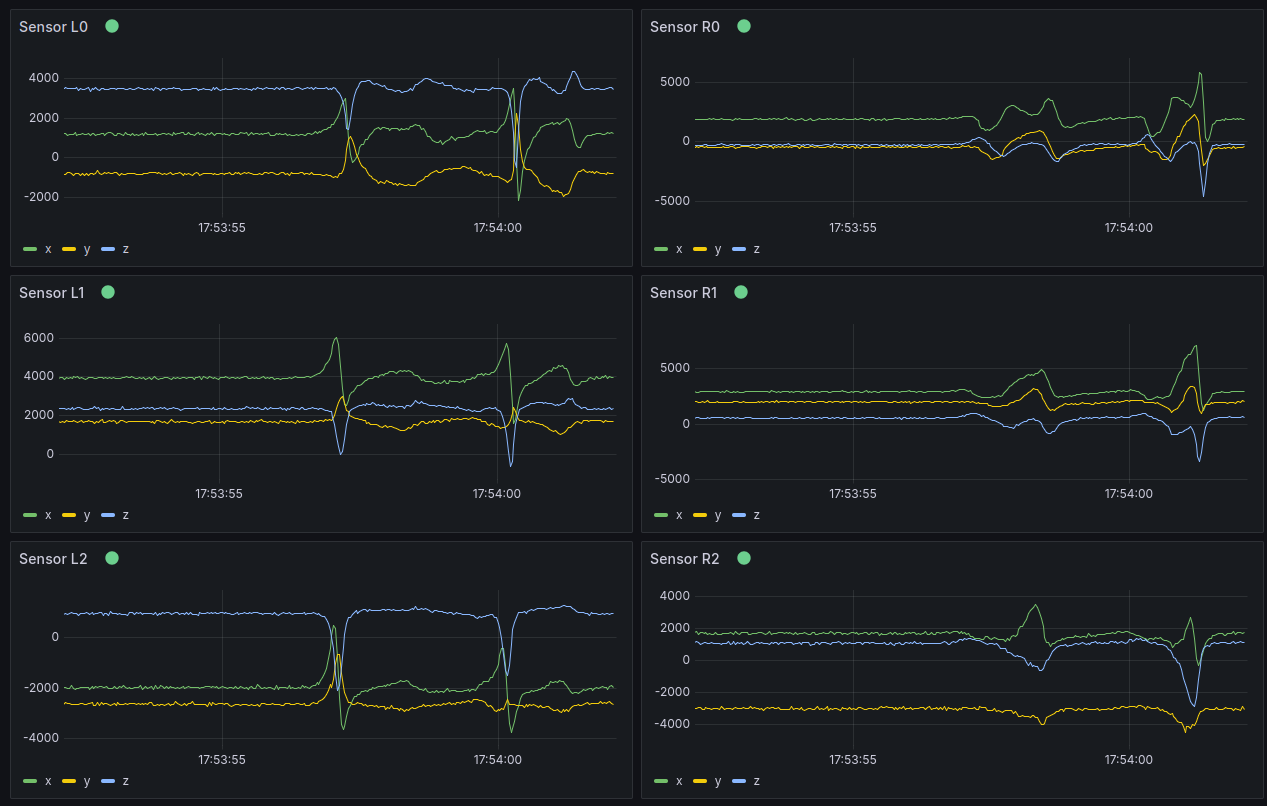
\includegraphics[width=\textwidth]{figures/grafana}
    \caption{visualization of magnetic data of 6 whisker sensors in real-time using Grafana.}
    \label{fig:grafana}
\end{figure}

The plans for the dashboard include:
\begin{itemize}
    \item Visualization of whisker deflection in 2D
    \item State machine visualization
    \item Performance metrics of the contour reconstruction algorithm
    \item System cycle time and overload monitoring
    \item Historical data analysis and trend monitoring.
\end{itemize}

    % !TeX spellcheck = en_US


\chapter{Conclusion}

\section{Summary}

\begin{enumerate}
    \item A \textbf{whisker array platform} for active tactile exploration was designed and assembled
    \item Control algorithms were implemented for:
    \begin{itemize}
        \item Contour reconstruction
        \item \textbf{Object retrieval}
        \item \textbf{Navigation in tunnels}
    \end{itemize}
    \item A \textbf{test framework with physics simulation} was developed for the whisker control system
    \item A \textbf{system infrastructure} was developed for real-time sensor data visualization and evaluation
\end{enumerate}

\section{Future Work}
\begin{itemize}
    \item Testing of the whisker control system with the Franka Emika Panda robotic arm
    \item Addition of more whiskers to each side of the platform
    \item Active exploration of unstructured environments
    \item SLAM for navigation in cluttered environments
    \item Integration of the whiskers into the robotic rat
\end{itemize}


    % Appendix
    \appendix
    \chapter{Appendix 1}
<Appendix 1>


    % References
    {
    %\sloppy% "Word"-like typesetting in order to improve breaking lines with long URLs/DOIs
        \printbibliography[heading=bibintoc]%
    }

\end{document}
